%
% exemplo genérico de uso da classe iiufrgs.cls
% $Id: iiufrgs.tex,v 1.1.1.1 2005/01/18 23:54:42 avila Exp $
%
% This is an example file and is hereby explicitly put in the
% public domain.
%
%TODO: Think of printing format
\documentclass[tuberlin,cic,tc,english,noabntcite]{iiufrgs}
% Para usar o modelo, deve-se informar o programa e o tipo de documento.
% Programas :
% * cic       -- Graduação em Ciência da Computação
% * ecp       -- Graduação em Ciência da Computação
% * ppgc      -- Programa de Pós Graduação em Computação
% * pgmigro   -- Programa de Pós Graduação em Microeletrônica
% * tuberlin  -- Bachelorarbeit entregue na TU Berlin
%
% Tipos de Documento:
% * tc                -- Trabalhos de Conclusão (apenas cic e ecp)
% * diss ou mestrado  -- Dissertações de Mestrado (ppgc e pgmicro)
% * tese ou doutorado -- Teses de Doutorado (ppgc e pgmicro)
% * ti                -- Trabalho Individual (ppgc e pgmicro)
%
% Outras Opções:
% * english    -- para textos em inglês
% * openright  -- Força início de capítulos em páginas ímpares (padrão da
% biblioteca)
% * oneside    -- Desliga frente-e-verso
% * nominatalocal -- Lê os dados da nominata do arquivo nominatalocal.def


% Use unicode
\usepackage[utf8]{inputenc}   % pacote para acentuação

% Necessário para incluir figuras
\usepackage{graphicx}         % pacote para importar figuras
\graphicspath{ {img/} }

\usepackage{times}            % pacote para usar fonte Adobe Times
% \usepackage{palatino}
% \usepackage{mathptmx}       % p/ usar fonte Adobe Times nas fórmulas

%\usepackage[alf,abnt-emphasize=bf]{abntex2cite}	% pacote para usar citações abnt
\usepackage[round]{natbib}

\usepackage{subcaption} %Support for sub figures
\usepackage{listings}
\usepackage{float}
\setlength{\intextsep}{1\baselineskip} % evita espaços antes e depois de floats
\usepackage{color}

\definecolor{mygreen}{rgb}{0,0.6,0}
\definecolor{mygray}{rgb}{0.5,0.5,0.5}
\definecolor{mymauve}{rgb}{0.58,0,0.82}

%\color{blue} %Printing work out

\lstset{ %
  backgroundcolor=\color{white},   % choose the background color; you must add \usepackage{color} or \usepackage{xcolor}
  basicstyle=\footnotesize,        % the size of the fonts that are used for the code
  breakatwhitespace=false,         % sets if automatic breaks should only happen at whitespace
  breaklines=true,                 % sets automatic line breaking
  captionpos=b,                    % sets the caption-position to bottom
  commentstyle=\color{mygreen},    % comment style
  deletekeywords={},            % if you want to delete keywords from the given language
  escapeinside={\%*}{*)},          % if you want to add LaTeX within your code
  extendedchars=true,              % lets you use non-ASCII characters; for 8-bits encodings only, does not work with UTF-8
  frame=single,	                   % adds a frame around the code
  keepspaces=true,                 % keeps spaces in text, useful for keeping indentation of code (possibly needs columns=flexible)
  keywordstyle=\color{blue},       % keyword style
  language=C,                 % the language of the code 
  otherkeywords={algorithm, for, each, if, then, do, endif, endfor, end, return, :=, not, empty},           % if you want to add more keywords to the set
  numbers=left,                    % where to put the line-numbers; possible values are (none, left, right)
  numbersep=5pt,                   % how far the line-numbers are from the code
  numberstyle=\tiny\color{mygray}, % the style that is used for the line-numbers
  rulecolor=\color{black},         % if not set, the frame-color may be changed on line-breaks within not-black text (e.g. comments (green here))
  showspaces=false,                % show spaces everywhere adding particular underscores; it overrides 'showstringspaces'
  showstringspaces=false,          % underline spaces within strings only
  showtabs=false,                  % show tabs within strings adding particular underscores
  stepnumber=1,                    % the step between two line-numbers. If it's 1, each line will be numbered
  stringstyle=\color{mymauve},     % string literal style
  tabsize=2,	                   % sets default tabsize to 2 spaces
  %caption=\lstname                   % show the filename of files included with \lstinputlisting; also try caption instead of title
}

%
% Informações gerais
%
\title{Towards Synchronizing Relations Between Artifacts in the Java Technological Space}

\author{Bombardelli da Silva}{William}
% alguns documentos podem ter varios autores:
% \author{Flaumann}{Frida Gutenberg}
% \author{Flaumann}{Klaus Gutenberg}

% orientador e co-orientador são opcionais (não diga isso pra eles :))
\advisor[Prof. Dr.]{Trollmann}{Frank}
\reviewer[Prof. Dr. Dr. h.c.]{Albayrak}{Sahin}
\reviewer[Prof. Dr. habil.]{Kao}{Odej}
%\coadvisor[Prof.~Dr.]{Knuth}{Donald Ervin}

% a data deve ser a da defesa; se nao especificada, são gerados
% mes e ano correntes
% \date{maio}{2001}

% o local de realização do trabalho pode ser especificado (ex. para TCs)
% com o comando \location:
\location{Berlin}{Germany}

% itens individuais da nominata podem ser redefinidos com os comandos
% abaixo:
% \renewcommand{\nominataReit}{Prof\textsuperscript{a}.~Wrana Maria Panizzi}
% \renewcommand{\nominataReitname}{Reitora}
% \renewcommand{\nominataPRE}{Prof.~Jos{\'e} Carlos Ferraz Hennemann}
% \renewcommand{\nominataPREname}{Pr{\'o}-Reitor de Ensino}
% \renewcommand{\nominataPRAPG}{Prof\textsuperscript{a}.~Joc{\'e}lia Grazia}
% \renewcommand{\nominataPRAPGname}{Pr{\'o}-Reitora Adjunta de P{\'o}s-Gradua{\c{c}}{\~a}o}
% \renewcommand{\nominataDir}{Prof.~Philippe Olivier Alexandre Navaux}
% \renewcommand{\nominataDirname}{Diretor do Instituto de Inform{\'a}tica}
% \renewcommand{\nominataCoord}{Prof.~Carlos Alberto Heuser}
% \renewcommand{\nominataCoordname}{Coordenador do PPGC}
% \renewcommand{\nominataBibchefe}{Beatriz Regina Bastos Haro}
% \renewcommand{\nominataBibchefename}{Bibliotec{\'a}ria-chefe do Instituto de Inform{\'a}tica}
% \renewcommand{\nominataChefeINA}{Prof.~Jos{\'e} Valdeni de Lima}
% \renewcommand{\nominataChefeINAname}{Chefe do \deptINA}
% \renewcommand{\nominataChefeINT}{Prof.~Leila Ribeiro}
% \renewcommand{\nominataChefeINTname}{Chefe do \deptINT}

% A seguir são apresentados comandos específicos para alguns
% tipos de documentos.

% Relatório de Pesquisa [rp]:
% \rp{123}             % numero do rp
% \financ{CNPq, CAPES} % orgaos financiadores

% Trabalho Individual [ti]:
% \ti{123}     % numero do TI
% \ti[II]{456} % no caso de ser o segundo TI

% Monografias de Especialização [espec]:
% \espec{Redes e Sistemas Distribuídos}      % nome do curso
% \coord[Profa.~Dra.]{Weber}{Taisy da Silva} % coordenador do curso
% \dept{INA}                                 % departamento relacionado

%
% palavras-chave
% iniciar todas com letras minúsculas, exceto no caso de abreviaturas
%
\keyword{Model Synchronization}
\keyword{Java Metamodels}
\keyword{Network of Models}
\keyword{Iterative Model Transformation}
\keyword{Model Transformation}
\keyword{Model-driven Engineering}
\keyword{Software Engineering}

%\settowidth{\seclen}{1.10~}

%
% inicio do documento
%
\begin{document}

% folha de rosto
% às vezes é necessário redefinir algum comando logo antes de produzir
% a folha de rosto:
% \renewcommand{\coordname}{Coordenadora do Curso}
\maketitle

% dedicatoria
% \clearpage
% \begin{flushright}
%     \mbox{}\vfill
%     {\sffamily\itshape
%       ``If I have seen farther than others,\\
%       it is because I stood on the shoulders of giants.''\\}
%     --- \textsc{Sir~Isaac Newton}
% \end{flushright}

% agradecimentos
\chapter*{Acknowledgments}
....



% resumo na língua do documento
\begin{abstract}
The use of models in software engineering processes has grown in the last few years. And as it grows, grows also the relevance of some problems related to the realm. One of them is the model synchronization problem, that consists basically of keeping all the models of a software system consistent between themselves. In other words, the models of a software tend to be changed over its lifetime, and as it happens, these changes have to be forwarded properly to all the models regarded to this software. For big programs it is clearly inviable to do such synchronization procedure manually, therefore it is desired the creation of automatic methods able to perform synchronization.

This thesis aim to (1) identify models of the Java technological space, (2) define some (or simplified versions) of them formally, (3) identify and formalize some relations between them, creating a network of metamodels supposed to be kept synchronized, and show through a representative showcase how they work, and finally (4) discuss the synchronization of this network of models. The outcomes include the implementation of these relations plus the report about the experience of developing it in this thesis.
\end{abstract}

% resumo na outra língua
% como parametros devem ser passados o titulo e as palavras-chave
% na outra língua, separadas por vírgulas
\begin{englishabstract}{Zur Synchronisation von Relationen Zwischen Artefakten im Java Technologischen Raum}{Modell-Synchronisation, Java Metamodelle, Netzwerk von Modellen, Iterative Modell-Transformation, Modell-Transformation, Modellorientierte Technik, Softwaretechnik}

Die Anwendung von Modellen in Softwaretechnikprozessen hat in der letzten Jahren gewachsen. Als es zunimmt, nimmt auch die Relevanz eigener auf den Bereich bezogenen Probleme zu. Ein davon ist das Modell-Synchronisationsproblem, das grundsätzlich aus dem konsistenten Bewahren von allen Modellen eines Softwaresystems besteht. Anders ausgedrückt tendieren die Modelle einer Software dazu, im Laufe der Zeit verändert zu werden. Wenn das vorkommt, müssen diese Veränderungen richtig nach allen Modellen weitergeleitet werden. Für größere Programme ist es offensichtlich unmöglich, solches Synchronisationsverfahren manuell zu unternehmen. Daher ist es wünschenswert, die Schaffung von automatischen Verfahren, die in der Lage sind, Synchronisation durchzuführen.

Diese Bachelorarbeit hat als Ziele (1) Modelle des Java technologischen Raums zu identifizieren; (2) einige davon formal zu definieren; (3) einige Relationen zwischen denen zu identifizieren und formalisieren, indem ein Netzwerk von Metamodellen aufgebaut wird, das synchronisiert aufbewahrt werden soll, und ein repräsentatives Beispiel gezeigt wird; und schließlich (4) die Synchronisation dieses Netzwerkes von Modellen zu diskutieren. Die Ergebnisse umfassen sowohl die Implementation dieser Relationen, als auch den Bericht über die Erfahrung der vorliegenden Bachelorarbeit.
\end{englishabstract}

% lista de figuras
\listoffigures

% lista de tabelas
%\listoftables

% lista de abreviaturas e siglas
% o parametro deve ser a abreviatura mais longa
\begin{listofabbrv}{MDSD}
	\item[ATL] Atlas Transformation Language
	\item[EMF] Eclipse Modeling Framework
	\item[HTML] Hypertext Markup Language
	\item[IDE] Integrated Development Environment
	\item[LHS] Left-hand Side
	\item[MDE] Model-driven Engineering
	\item[MDSD] Model-driven Software Development
	\item[MOF] Meta-Object Facility
	\item[RHS] Right-hand Side
	\item[SUS] System Under Study
    \item[TGG] Triple Graph Grammar
    \item[UML] Unified Modeling Language
\end{listofabbrv}

% idem para a lista de símbolos
% \begin{listofsymbols}{$\alpha\beta\pi\omega$}
%     \item[$\sum{\frac{a}{b}}$] Somatório do produtório
%     \item[$\alpha\beta\pi\omega$] Fator de inconstância do resultado
% \end{listofsymbols}

% sumario
\tableofcontents

%%%%%%%%%%%%%%%%%%%%%%%%%%%%%%%%%%%%%%%%%%%%%%%%%%%%%%%%%%%%%%%%%%%%%%%%
% Chapter
%%%%%%%%%%%%%%%%%%%%%%%%%%%%%%%%%%%%%%%%%%%%%%%%%%%%%%%%%%%%%%%%%%%%%%%%
\chapter{Introduction}
The techniques for software development has changed in the course of time since the rise of general-purpose programmable computers and specially in the second half of the 20th century with the rise of digital computers \citep{ceruzzi2003history}. In the beginning of digital computer programming, machine code was used to describe algorithms, but as the complexity and the size of such algorithms got bigger, this technique soon became impracticable, what evoked the need for a more sophisticated way of programming these digital machines. The assembly languages (also known as low-level programming languages) came to solve this problem, but clearly the complexity kept increasing as well as the need for new techniques and technologies for software programming. The popularization of computing and the increasing application of computers in the practice urged the creation of high-level programming languages (e.g. Cobol, Fortran), which kept evolving mainly in regard to the needs of the software market \citep{ceruzzi2003history}. More sophisticated languages (e.g. C, Pascal) and new paradigms (e.g. modular and object-oriented programming) also arose in the late 20th century. But the evolution of software development does not seem to stop, evidenced by the lately increasing research on new software engineering techniques such as the Model-driven Engineering.

The newest characteristics of the information system market, like the constant evolution of the software systems, the interoperability between them and the big number of developers working in a common software artifact has required the use of software models and, consequently, the research on how to apply them systematically and correctly in the development processes, the so-called Model-driven Engineering (MDE) or Model-driven Software Development (MDSD) \citep{france2007model}. This Bachelor thesis aims, therefore, to explore one specific realm of Model-driven Engineering research, namely the problem of synchronization of models (or artifacts) in the Java technological space. The goal here is to pick commonly used metamodels in Java systems, describe them and identify their relations, so that they can be synchronized.

The remainder of this document is structured in 7 chapters. The first chapter introduces the scope and defines the problem dealt by this thesis. The second chapter presents a literature review comprising the basic definition necessary for the further development of the text. Chapter 3 shows the current stage of scientific research related to the field of this work. Chapter 4 presents the developed metamodels and the relations between, whereas the chapter 5 proposes an algorithm for the synchronization of models. Finally, chapter 6 and 7 discuss the results and give an overview of the work.

%---------------------------------------------
% Section
%---------------------------------------------
\section{Background}
According to \citet[p. 21]{czarnecki2006feature}: "\textit{Models are system abstractions that allow developers and other stakeholders to effectively address concerns, such as answering a question about the system or effecting a change}”. By defining a model as a system abstraction, it becomes clear, that a software system might have several models abstracted from it, each one representing certain aspects of the whole system. These models also have relations between them, in the sense that they all are supposed to describe the actual system consistently by not presenting logical contradictions. Here examples of models are \emph{UML class diagram}, \emph{Use Cases}, or even the source-code itself. The term model and artifacts will be used interchangeably throughout this document.

The constant evolving nature of current large-scale software systems causes their models to be constantly changed \citep{diskin2011model}. But in order to maintain this whole network of interconnected models consistent, the changes have to be forwarded through the network, i.e. all models have to be synchronized. Suppose one have a \emph{UML Class Diagram}, a series of \emph{UML Sequence Diagrams} and the source-code. If a method has its name changed in the class diagram, all occurrences of this method have to have their name updated in the sequence diagrams and in the source-code. It turns out though, that neither a model synchronization tool comprising the most common metamodels used nowadays in Java information systems is known by us, nor have we found clearly defined relation definitions between them on the literature, even though an expressive effort has been made by the academic community to create solutions for the problem of model synchronization. 

%---------------------------------------------
% Section
%---------------------------------------------
\section{Motivation}
Problems of software quality, like security flaws, software not working according to its specification (i.e. bugs), or even performance questions are an issue of interest of both the industry and the academic community. Model-driven Engineering (MDE) claims to leverage the use of models in order to help bridge the gap between the problem and the implementation domains \citep{france2007model}, and therefore to reduce some problems of quality. This discussion points to the motivation of the use of models, but also highlights the need for synchronization methods, that allow the network of models of a system to be kept consistent. In fact, the synchronization could be done manually by the users, since they can a priori update all models related to the one under changes, but this manual process usually requires much time from expensive workforce and it is error-prone. Automated (or at least partially-automated) model synchronization endeavors to reach a higher reliability on the models, as well as lower costs for the software maintainer.

In general, synchronized models enhance the documentation quality, once many of them are used for documentation purposes; ease the act of evolving software, by bridging the gap between problem (abstract) and implementation (concrete) levels; and support the debugging processes, once models are used to consult information about the system under study. On the other hand, if one model is not kept consistent with another, it may lose its validity, once the information it addresses cannot be trusted anymore, and consequently the user cannot rely on it anymore. If the number of inconsistencies between models is large enough, the users run the risk of not being able to use a big part of their set of models, what itself lowers the quality of the software.

Generally, the amount of inconsistencies tend to grow as the size of a program grows. The complexity of the network of models, as well as of the synchronization task increases therefore too, what also gives reason to the application of more robust synchronization techniques. This phenomenon occurs specially in the case of a Java program, so Java is used in this thesis as an example domain.

%---------------------------------------------
% Section
%---------------------------------------------
\section{Objective}
This bachelor thesis aims to (1) present some artifacts from the Java technological space, that might require synchronization, explaining their objectives and some basic elements from them; (2) formalize and explain the relations between these artifacts, so that the synchronization is possible; and finally (3) discuss how synchronization may be accomplished in a representative showcase.

This document presents the documentation of the three objectives mentioned before. Furthermore, the report of the difficulties and experiences found during the work process and an examination of possible future development and challenges of the realm is also a goal.


%---------------------------------------------
% Section
%---------------------------------------------
\section{Methodology}
In order to achieve the goals, the following procedure is taken. In the first moment a collection of common metamodels used in the Java technological space is to be defined, this is done through an state-of-art research, since that some metamodels have already been defined by other authors, plus the creation of our own versions of some metamodels. So for example, in this phase the choice of the applied metamodels (i.e. \emph{UML Class Diagram} and \emph{Java Code}) is done and their definitions are written.

Later on, given the defined metamodels, the relations between them can be written. So for example, in this phase the inherent relation between the \emph{UML Class Diagram} metamodel and the \emph{Java Code} metamodel is written. Analogously, the relations between \emph{Java Code} and other metamodels of the Java technological space are also to be defined. All of these relations are developed during the work of this thesis.

After having this network of metamodels ready, a showcase using a transformation method from the current academic literature is applied to illustrate how the relations between the metamodels work. We work therefore with the hypothesis, that the metamodels can be found or defined; that some relations between them can be written in some language; and that some of these relations can be transformed using a tool or technique available in the current literature.

It is out of the scope of this work the creation of complete metamodel definitions, or relations, or the implementation of a full-working synchronization algorithm. A deep theoretic analysis about the problem or about the performance of the relations is also excluded from this scope.

%%%%%%%%%%%%%%%%%%%%%%%%%%%%%%%%%%%%%%%%%%%%%%%%%%%%%%%%%%%%%%%%%%%%%%%%
% Chapter
%%%%%%%%%%%%%%%%%%%%%%%%%%%%%%%%%%%%%%%%%%%%%%%%%%%%%%%%%%%%%%%%%%%%%%%%
\chapter{Foundations}
\label{ch:foundations}
Before describing the development of this thesis, it is important to review some important definitions regarded to Model-driven Engineering. Below is a list of necessary basic concept definitions, that will be used throughout this document. Some of these definitions are rather narrower than they could be, but for the scope of this thesis they seem to be suitable.

\begin{description}
	\item[Technological Space:] According to the definition from \citet[p. 1]{kurtev2002technological}: \emph{"A technological space is a working context with a set of associated concepts, body of knowledge, tools, required skills, and possibilities. It is often associated to a given user community with shared know-how, educational support, common literature and even workshop and conference meetings"}. By Java Technological Space it is meant the set of commonly used models, practices, techniques and technologies in Java software development. For example, object-oriented development, unit tests, code documentation and the \emph{Java Virtual Machine} are items of the Java technological space.

	\item[System:] \emph{"A system is the primary element of discourse when talking about MDE."} \citep[p. 13]{favre2004foundations}. One example of a system, according to this definition, is a Java program, once it can be the primary handled element in a certain software engineering context. Nevertheless, this definition is wide enough to affirm that a \emph{UML Class Diagram} is a system, since it can be the primary handled element in a certain context. This fact allows an easier-to-understand definition of model.

	\item[Model:] According to \citet{favre2004foundations}, a model is a possible role a system can play. A system plays the role of a model, when it represents another system (system under study, or SUS). By being so, when one refers to the a model $M$, it is meant, a system that represents (or abstracts) another system $S$, i.e. $M \mu S$. \citet{seidewitz2003models} affirms that, models can be used (1) to describe a system, in this case the model makes statements about the SUS, an example is an \emph{UML sequence diagram} employed to help understand the behavior of a Java program. But models can also be used (2) to specify a system, in this case it is used in the validation of the system, an example is a \emph{UML class diagram} employed as design specification of a Java system. Further examples of models, according to this definition, are a \emph{relational database diagram} of a database, the documentation of a system in \emph{Java Doc} or even a Java source-code.

	\item[Modeling Language:] A model is expressed, using a modeling language. \emph{"A modeling language (L) is a set of models"} \citep[p. 13]{favre2004foundations}, that contains all the models $M_i$ expressed in that language, i.e. $L \owns M_i$. Examples of modeling languages are the \emph{UML}, the \emph{diagram notation for relational database diagram} or the Java language.

	\item[Metamodel:] \citet[p. 14]{favre2004foundations2} affirms also: \emph{"A metamodel is a model of a modelling language."}. In other words, a metamodel specifies what can be written using a certain modeling language. One certain model $M$ is conform to a meta-metamodel $MM$ (i.e $M \epsilon MM$), if and only if, $M \in L$ and $MM \mu L$. Thus, examples of metamodels are \emph{UML specification document} \citep{omg2007unified}, the \emph{entity-relationship metamodel} \citep{chen1976entity} or the Java metamodel (one example is to be found in \citet{heidenreich2009jamopp}). Finally \citet[p. 29]{seidewitz2003models} also claims: \emph{"Because a metamodel is a model, we express it in some modeling language"}. One example of a modeling language for metamodels is the \emph{EMF Ecore}\footnote{https://eclipse.org/modeling/emf} (which is the modeling language for metamodels used in this thesis and is explained further below).
	
	\begin{figure}[H]
		\caption{The summary of the definitions of system, model, metamodel, meta-metamodel and modeling language.}
		\centering
		\begin{subfigure}[h]{.3\textwidth}
   			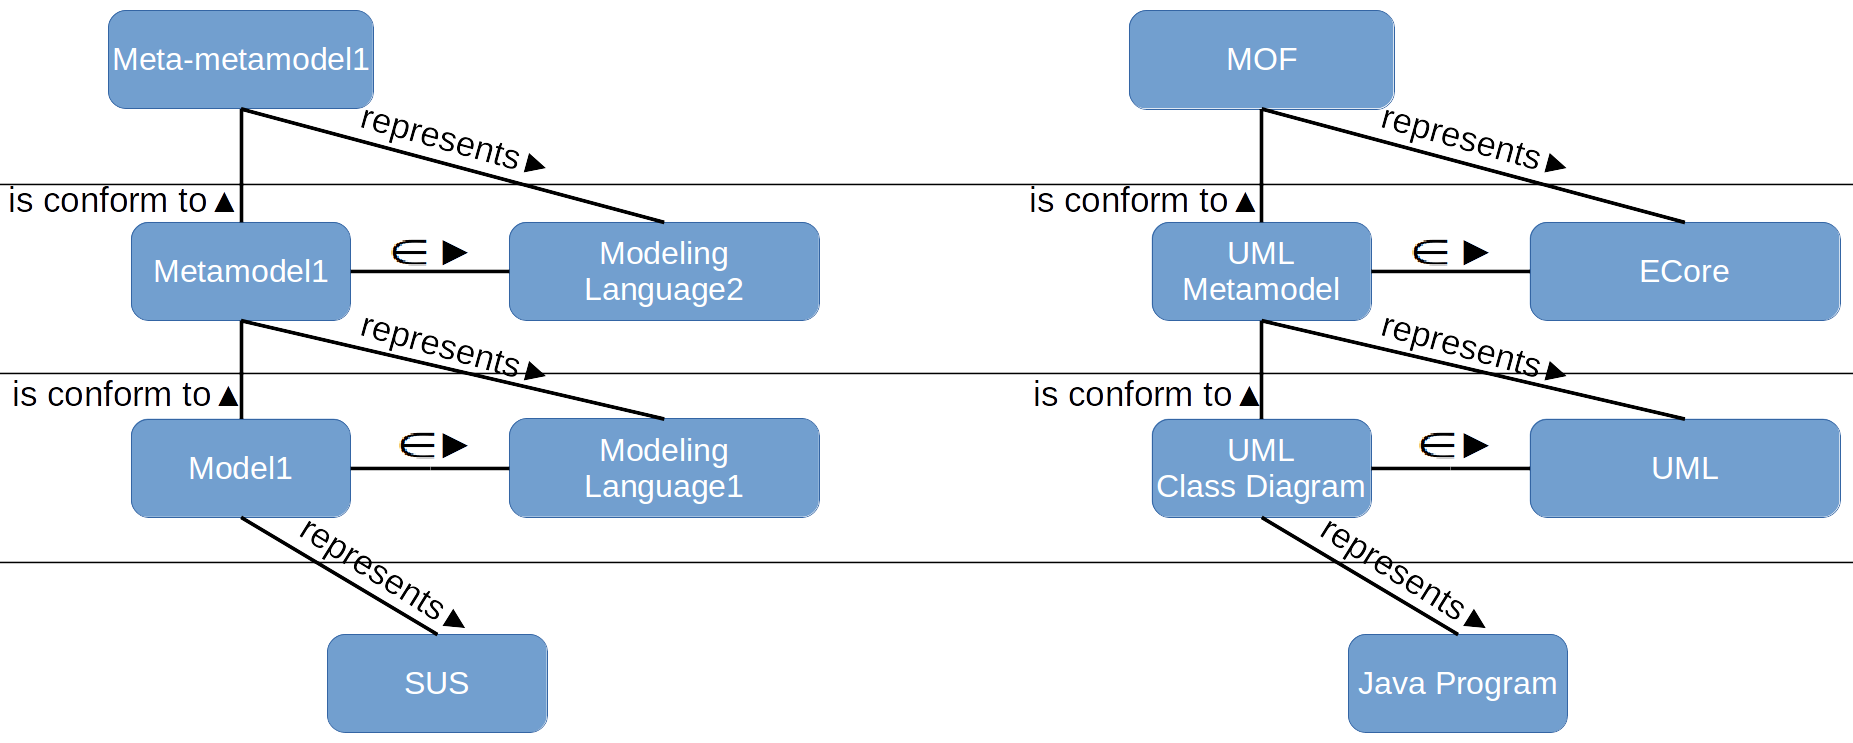
\includegraphics[width=\textwidth]{model_scheme}
		\end{subfigure}
		\begin{subfigure}[h]{.3\textwidth}
			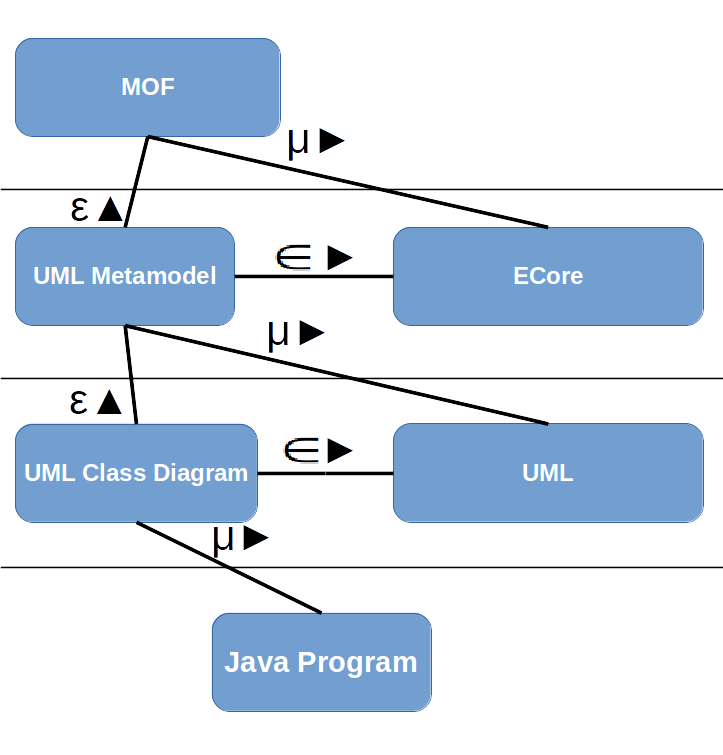
\includegraphics[width=\textwidth]{model_scheme_practice}
		\end{subfigure}
		\label{fig:model_scheme}
		\legend{Source: The author}
	\end{figure}

	\item[Meta-metamodel:] Analogously to the metamodel definition, one can go forth and define meta-metamodel, which is a model that specifies a modelling language for metamodels. An example of meta-metamodel is the \emph{MOF}\citep{omg2015meta}, which the \emph{EMF Ecore} is conform to. It is to note also, that such derivation can be done iteratively in the sense that a $meta^3model$ definition is also possible, although it is not useful for the scope of this thesis. The Figure \ref{fig:model_scheme} illustrate our understanding of the definitions above. On the left is a depiction of the theoretical definitions of system, model, metamodel, meta-metamodel and modeling language. Like stated before, a system is represented by models, which themselves are expressed in languages and are conform to metamodels. A more concrete and practical illustration of the definitions is on the right. This example shows a scenario very close to the implementation made in chapter \ref{chapter:metamodel_relations}.
	
	\item[Model Relation:] Model relation here is defined abstractly as every relationship or constraint possible to happen between one source model and one target model. For instance, the models \emph{UML class diagram} and Java code have a relation, because once a new class is created in the class diagram, the correspondent class has to be created in the Java code. Moreover, a \emph{UML class diagram} with contract definitions (pre and post-conditions) have a relation to the \emph{JUnit} model, once that the formers have to be tested correspondingly in the latter.

	\item[Model Transformation:] Model transformation can be viewed as common data transformation – very common in computer science – with the specificity of dealing with models \citep{czarnecki2006feature}. More specifically, model transformation is defined here as a function $t : M \rightarrow N$, where $t(m) = n$ means that a target model $n \in N$ is created from a source model $m \in M$, $M$ and $N$ being respectively the set of all valid models of the metamodels $\Phi_M$ and $\Phi_N$. Practical example: Creation of Java code from \emph{UML class diagram}. Note that, model transformation is by nature deterministic, unidirectional and does not preserve the information of the target model (e.g. comments in the Java code).

	\item[Model Synchronization:] The goal of model synchronization is to maintain all relations between the models of a system consistent/correct, as updates are performed over them \cite{diskin2011model}. More specifically, model synchronization is defined here as a function $s : M \times M \times \Delta_M \times N \times N \times \Delta_M \rightarrow M \times N $, where $s(m_0,m_1,\delta_m,n_0,n_1,\delta_n) = (m_2,n_2)$ means that final synchronized models $m_2$ and $n_2$ are created from the initial synchronized models $m_0$ and $n_o$ and the modified non-synchronized models $m_1$ and $n_1$, considering the modifications (respectively $\delta_m$ and $\delta_n$) performed over both. Practical example: Modification of a method name ($\delta_m$) in the \emph{UML class diagram} ($m_0$) has to be forwarded to the Java code ($n_0$), without losing extra information of it (e.g. comments). Note that, model synchronization is deterministic, bidirectional and preserves the informations of the both models. Other terms for model synchronization are \emph{iterative} or \emph{information preserving bidirectional model transformation}.

	\item[Network of Models:] A network of models of a system $S$ is an undirected graph $G = (V,E)$, whereas each vertex $v_i \in V$ represents a unique model $i$ abstracting $S$, and an edge $(v_i, v_j)$ exists if, and only if there is a relation defined between both models $i$ and $j$. In the Figure \ref{fig:network_example_01} is an example of a network of models, illustrating the possible complexity of such network. More discussion is to find in \citet{mens2006taxonomy}.

	\begin{figure}[H]
	    \caption{An example of a network of models very similar to the one developed in this work.}
	    \begin{center}
	        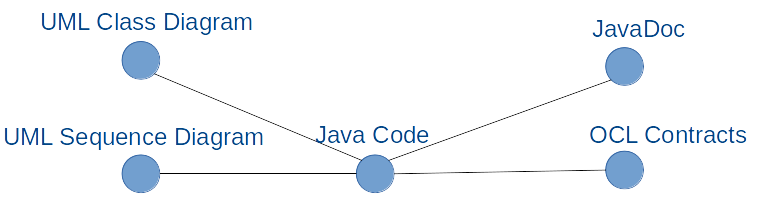
\includegraphics[width=25em]{network_example_01}   
	    \end{center}
	    \label{fig:network_example_01}
	    \legend{Source: The Author}
	\end{figure}

	\begin{figure}[H]
	    \caption{Part of MOF definition, which handles basically classes, properties, operations, associations, and generalization.}
	    \begin{center}
	        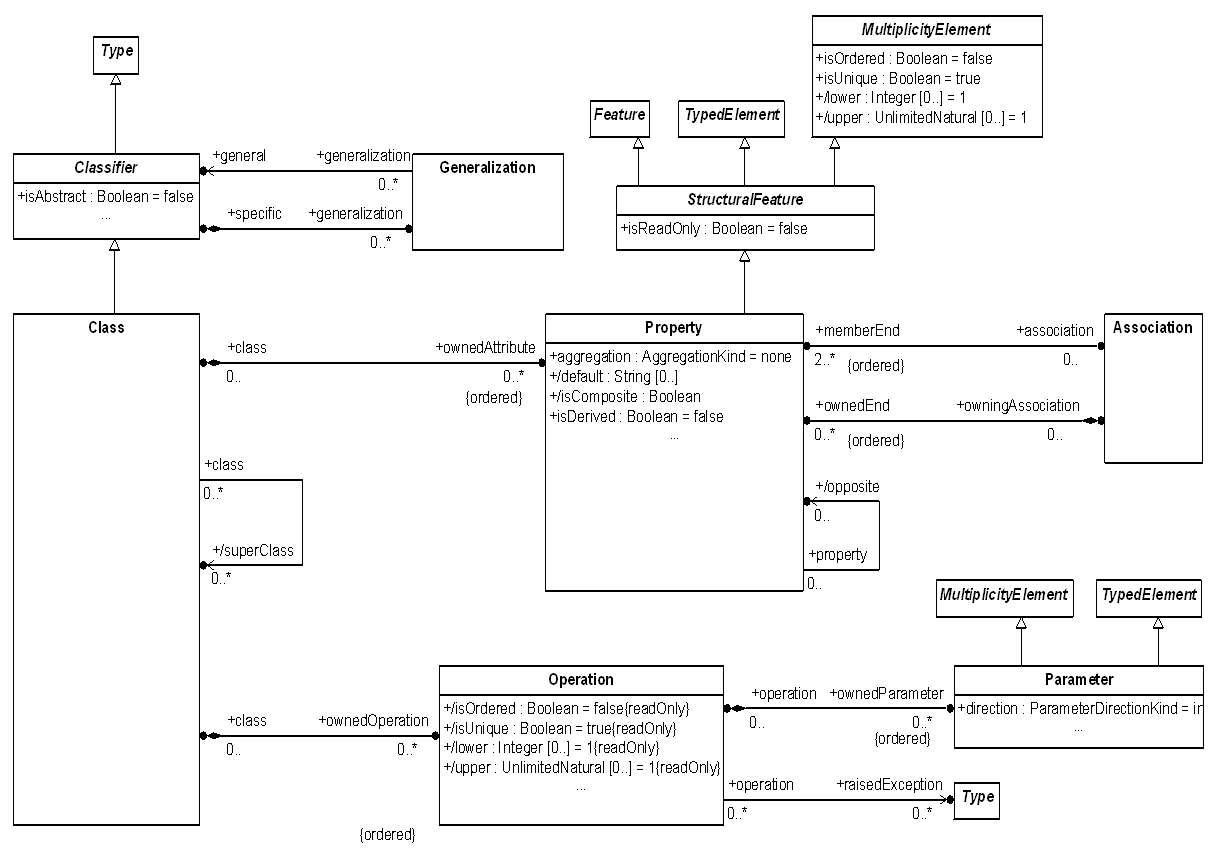
\includegraphics[width=.7\textwidth]{emof_classes}   
	    \end{center}
	    \label{fig:emof_classes}
	    \legend{Source: \citep[p. 27]{omg2015meta}}
	\end{figure}
	
	\item[Meta Object Facility:] \emph{"The Meta Object Facility (MOF) provides an open and platform-independent metadata management framework and associated set of metadata services to enable the development and interoperability of model and metadata driven systems"} \citep{omg2015meta}. The MOF describes therefore the MOF modeling language. Essentially, it inherits much from the UML and deals with the ideas of classes, properties and associations, providing and extensible but simple fashion to define metamodels. The Figure \ref{fig:emof_classes} shows one part of MOF.
	

	\item[Ecore:] Ecore\footnote{https://eclipse.org/modeling/emf} is the meta-metamodel utilized in this thesis to describe all the applied metamodels (e.g the Java metamodel). Ecore is an initiative of the EMF Project and aims to provide not only a meta-metamodel but a set of tools for creating metamodels, like an Eclipse plug-in generation feature, that enables the model developer to easily test and debug its metamodels. The Ecore meta-metamodel is very similar to the essential MOF standard. That is the reason, why it is applied here. A proof of such compliance is not know by us though. The Figure \ref{fig:ecore_relations} shows one part of Ecore.

	\begin{figure}[H]
	    \caption{Ecore definition illustrating the use of classes, attributes, operations, references and super types, analogously to the figure \ref{fig:emof_classes}}
	    \begin{center}
	        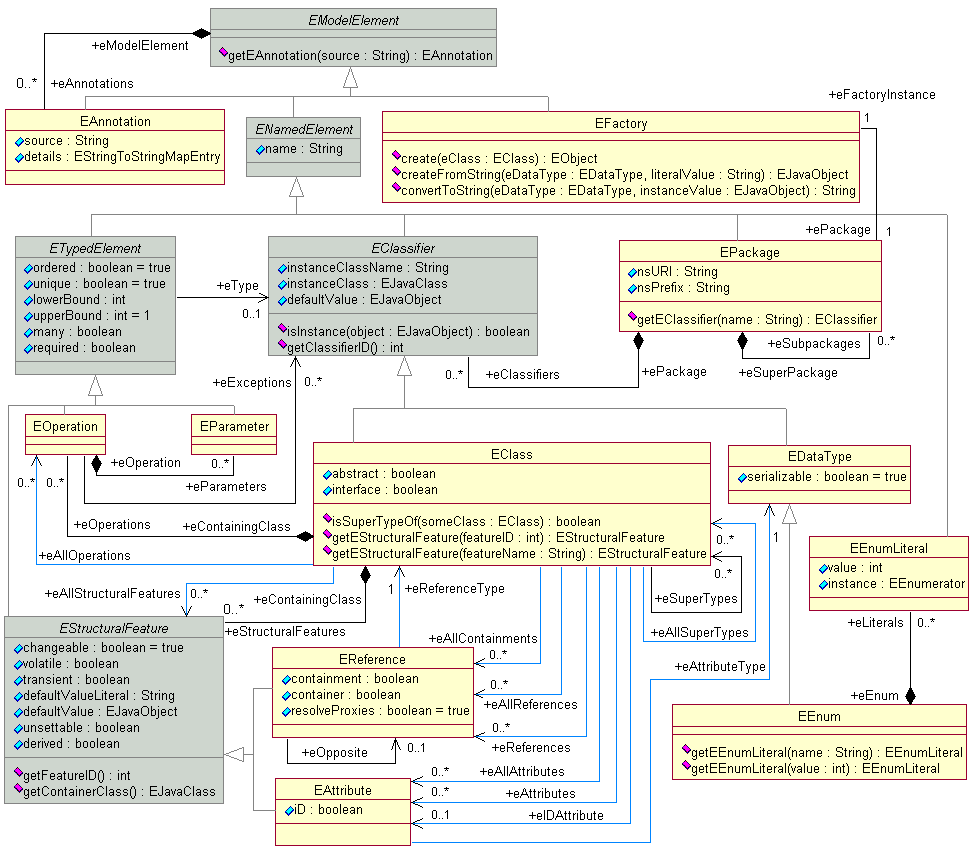
\includegraphics[width=.7\textwidth]{ecore_relations}   
	    \end{center}
	    \label{fig:ecore_relations}
	    \legend{Source: http://download.eclipse.org/modeling/emf/emf/javadoc/2.9.0/org/eclipse/emf/ecore/package-summary.html. On the December 29th, 2015}
	\end{figure}

	\item[Triple Graph:] With the use of a triple graph a relation between a source model $S$ and a target model $T$ are abstracted into a triple $(G_s,G_c,G_t)$ – where $G_s$ is the graph representation of source model elements, $G_t$ is the graph representation of target model elements, and $G_c$ represents the correspondence between the two set of model elements – together with two mappings $s_g: G_c \rightarrow G_s$ and $t_g: G_c \rightarrow G_t$, which bind the three graphs \citep{hermann2011correctness}.
	
	In this case, an addition in the triple graph $G = (G_s,G_c,G_t)$, that leads to a new triple graph $H = (H_s,H_c,H_t)$ consists in a triple graph morphism $m: G \rightarrow H$, with $m = (m_s,m_c,m_t)$. According to the Figure \ref{fig:tg_morphism}.

	\begin{figure}[h]
	    \caption{The morphism $m: G \rightarrow H$ is a triple graph $m = (m_s,m_c,m_t)$.}
	    \begin{center}
	        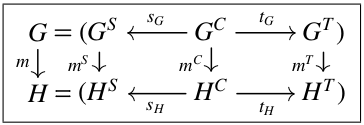
\includegraphics[width=15em]{tg_morphism}   
	    \end{center}
	    \label{fig:tg_morphism}
	    \legend{Source: \citep{hermann2011correctness}}
	\end{figure}

	\item[Triple Rule:] A triple rule is a triple graph morphism $t_r = (s, c, t) : L \rightarrow R$, where $L$ and $R$ are called respectively the left-hand the right-hand sides (respectively LHS and RHS) \citep{ehrig2007information}.
	
	\begin{figure}[H]
		    \caption{An example of two triple rules}
		    \label{fig:tgg_axiom_rule}
		    \centering
		    \begin{subfigure}{.7\textwidth}
			    \caption{Triple axiom example for a relation between \emph{UML} and \emph{Java}}
		        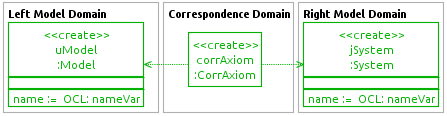
\includegraphics[width=\textwidth]{tgg_axiom} 
		        \label{fig:tgg_axiom}  
		    \end{subfigure}
		    \begin{subfigure}{.7\textwidth}
			    \caption{Triple rule example for a relation between \emph{UML} and \emph{Java}}
		        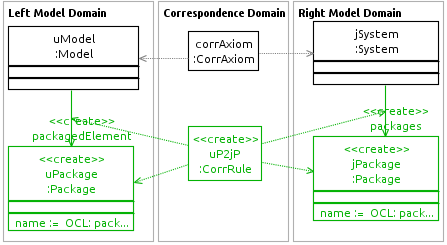
\includegraphics[width=\textwidth]{tgg_rule} 
		        \label{fig:tgg_rule}  
		    \end{subfigure}
		    \legend{Source: The author}
		\end{figure}
		
	\item[Triple Axiom:] A triple axiom is a triple rule $t_a = (s, c, t) : \emptyset \rightarrow R$. In order to represent triple graphs, it is common to use attributed graphs together with an easier-to-read diagram scheme, that comprises three columns (left model domain, correspondence domain, and right model domain) each one representing respectively the source model elements, the correspondence between source and target and, finally, the target model elements. A triple rule in turn is represented by a triple graph in black (left-hand side) plus a triple graph in green (right-hand side) (see \ref{fig:tgg_rule}). Because an axiom is a triple rule with empty left-hand side, only green graph occurs in an axiom (see \ref{fig:tgg_axiom}).

	\item[Triple Graph Grammar:] A triple graph grammar $TGG = (t_a, T_{rules}) $ consists of a triple axiom $t_a$ and a set of triple rules $T_{rules}$ \citep[p. 4]{giese2010toward}. While one triple graph can be used as a description of a relation between two metamodels, one TGG describes the language of the these two related models and serves rather as description of consistency. Nevertheless, extra rules can be derived from a TGG, in order to create the operational semantic of a transformation procedure \citep{giese2010toward}. Figure \ref{fig:transformation_scheme} summarizes the definitions of model relation, transformation and synchronization as well as triple graph grammars (TGG). The concept of modeling language is pictured as red lines.

	\begin{figure}[h]
	    \caption{Illustration of the terms of model relation, transformation and synchronization and triple graph grammars (TGG)}
	    \begin{center}
	        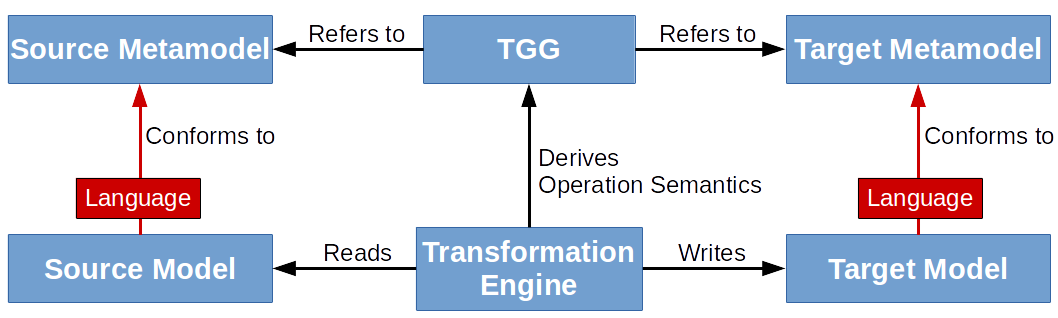
\includegraphics[width=.7\textwidth]{transformation_scheme}
	    \end{center}
	    \label{fig:transformation_scheme}
	    \legend{Source: Adapted from \citet[p. 623]{czarnecki2006feature}}
	\end{figure}
\end{description}

%---------------------------------------------
% Section
%---------------------------------------------
\chapter{State of the Art}
Some endeavors have been made in order to code relations between some metamodels and mainly to develop theoretical results and synchronization methods. \citeauthor{heidenreich2010closing} present in \citeyearpar{heidenreich2009jamopp} and \citeyearpar{heidenreich2010closing} a Java metamodel using \emph{Ecore}, what influences considerably the development of our work, although it is not directly used by us because of its size and unnecessary comprehensiveness for our needs. \citet{greenyer2008tggs} comes up with a transformation between \emph{UML activity diagrams} and \emph{CSP diagrams} using TGG. \citet{foss2011uml} define the translation between \emph{UML} and \emph{Simulink} using graph grammars. \citet{blouin2014synchronization} report about the synchronization between some specific metamodels of the automotive standards and influence our work, by using the same modeling language and transformation method as us, namely EMF \citep{steinberg2008emf} and \emph{MoTE} \citep{giese2010toward}. Finally \citet{giese2010model} introduce their approach to the synchronization of two automotive industry metamodels, lightening in the paper the \emph{MoTE} tool and its algorithm for synchronization.

We judge that the \emph{MoTE} transformation tool is the most adequate option for our needs, once literature about it is widely available (see also \citep{giese2009efficient} and \citep{hildebrandt2012mdelab}). Nevertheless there are other attempts to build a model synchronization tool, like the \emph{ATL Eclipse Plug-in} \citep{jouault2008atl}, which uses the \emph{Atlas Transformation Language} to code the relations between models; the Medini QVT \footnote{http://projects.ikv.de/qvt}, which claims to implement the \emph{Query/View/Transformation Language} to code the relations; and the FUJABA \citep{nickel2000fujaba}, in which relations are coded using TGG's. \citet{hildebrandt2013survey} also publicized a survey on synchronization tools based on TGG. Other publications aim to solve specific problems, like the ones in \citet{hermann2011correctness}, \citet{xiong2007towards}, \citet{giese2006incremental}, \citet{ivkovic2004tracing}, or \citet{song2011instant}, where advanced algorithms for bidirectional synchronization have been proposed.

A research road-map for model synchronization found in \citet{france2007model} gives an overview on the realm, and together with \citet{mattsson2009linking} show an interesting point of view about the challenges. \citet{seidewitz2003models} writes an interesting reflection  about what models mean and how to interpret them and in \citet{mens2006taxonomy} a taxonomy for model transformation is proposed, what helps to carry more precise analysis. In \citet{czarnecki2006feature} a survey was driven and a framework for classification of model transformation approaches was presented. In \citeauthor{diskin2014towards} \citeyearpar{diskin2014towards} and \citeyearpar{diskin2016three} a taxonomy for a network of models is presented and in \citet{diskin2011model} a theoretical algebraic basis is proposed.

Additionally, one can judge by the date of publication of these works, that the topic of model synchronization is extremely active and is actually the edge of current academic research, what motivates even more the development of this thesis.

%%%%%%%%%%%%%%%%%%%%%%%%%%%%%%%%%%%%%%%%%%%%%%%%%%%%%%%%%%%%%%%%%%%%%%%%
% Chapter
%%%%%%%%%%%%%%%%%%%%%%%%%%%%%%%%%%%%%%%%%%%%%%%%%%%%%%%%%%%%%%%%%%%%%%%%
\chapter{Metamodel Relations in the Java Technological Space}
\label{chapter:metamodel_relations}
With the terms and the theoretical basis clarified, the report of the main development phase of the thesis is shown below. The idea here is first to present the selected network of metamodels, by describing what each model represents and how they relate to each other. Then the developed metamodel definitions and the relations between them are exposed, as well as the justification of the choices made during the work. Attached to this thesis is the digital version of these metamodels and the definitions of the relations.

%---------------------------------------------
% Section
%---------------------------------------------
\section{Network of Metamodels}
The choice of which models are used in a certain Java program may vary considerably depending on the context of the development and the software requirements, which themselves can range from high dependability (e.g. airplane software) to continuous evolution (e.g. applications for cellphones), for example. Nevertheless, we select a few typical models plus the relations between them and create a network of metamodels. The Figure \ref{fig:network_metamodels} depicts this network. The bold printed vertices and edges represent respectively the metamodels and the relations, that are treated more deeply in this thesis, namely \emph{Java}, \emph{UMLClassDiagram}, \emph{UMLSequenceDiagram} and \emph{UMLContract}, whereas the other vertices are by virtue of the scope of this thesis some rather more briefly discussed metamodels, namely \emph{UMLUseCaseDiagram}, \emph{RequirementDiagram}, \emph{JavaDoc}, \emph{UnitTest}, \emph{UMLStateMachine}, \emph{ERDiagram}, \emph{FormalSpecification}.

\begin{figure}[H]
    \caption{A network of metamodels in the Java technological space}
    \begin{center}
        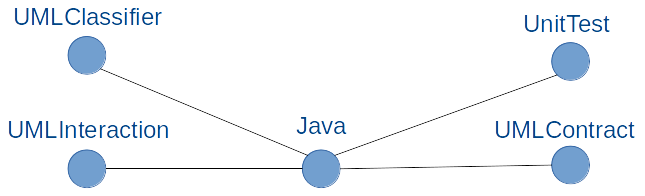
\includegraphics[width=.6\textwidth]{network_metamodels}
    \end{center}
    \label{fig:network_metamodels}
    \legend{Source: The author}
\end{figure}

The central element of the network is the \emph{Java} metamodel. A Java model (or, Java code) contains both structural and behavioral information about the system, which is represented among other elements through \emph{classes}, \emph{fields}, \emph{methods} and \emph{statements}.

Once a metamodel might be relatively big and comprise a huge number of elements, it is interesting to split it into smaller pieces for a specific set of relations. Take for example the UML, that includes a large number of different concerns (e.g. classifiers, state machines, activities, interaction, etc) and may be split into sub metamodels in order to ease the writing of the relations. For this reason, we separate the UML into \emph{UMLClassDiagram}, \emph{UMLSequenceDiagram}, \emph{UMLContract}, \emph{UMLUseCaseDiagram} and \emph{UMLStateMachineDiagram}. The first is constructed around the concepts of \emph{class}, \emph{property}, \emph{operation}, \emph{interface} and \emph{package}. This metamodel is usually used to describe the structure of an object-oriented Java program through a class diagram, representing the definition of its classes, fields and methods, but leaving out behavioral aspects. The relations between \emph{UMLClassDiagram} and \emph{Java} is then given by an almost direct translation between their elements. A \emph{class} in the former is transformed into a \emph{class} in the latter, a \emph{property} in a \emph{field}, an \emph{operation} in a \emph{method} and so on.

To represent some behavioral aspects, \emph{UMLSequenceDiagram} is used instead. The elements of this metamodel are usually reproduced with sequence diagrams, where \emph{lifelines} and \emph{messages} provide information about the sequence of event occurrences. In a Java program it may correspond to the sequence of calls inside a specific method. This means, the semantical information of each sequence diagram could be brought to the correspondent method in the Java model.

\emph{UMLContract} is based on the ideas of design-by-contract, whose main goal is to improve reliability of object-oriented software \citep{meyer1992applying}, and where operations have \emph{pre} and \emph{postconditions} as well as \emph{invariants}. Its relation with \emph{Java} is basically, that each constraint of the contracts can (1) be tested as assertions and (2) expressed in terms of annotations in the Java source-code. Moreover, one can have check methods in Java, which serve to verify the constraints of the class and, therefore, are supposed to be updated as soon as the contracts undergo changes. Related to contracts are also \emph{Formal Specifications}, these taking several different forms, among them the Z Notation \citep{spivey1992z}, which itself also refers to \emph{pre} and \emph{postconditions}.

The \emph{UnitTest} endeavors to enhance the software quality by means of tests. It tests small units of code, by basically verifying the pre and postconditions as well as invariants of each method. Because unit tests for Java programs are usually written in Java, we use the same metamodel for the vertices \emph{Java} and \emph{UnitTests} of our network. Anyways, the relation between both is based on creating \emph{test cases} in the latter according to the contract \emph{annotations} (e.g pre and postconditions, invariants, examples, etc) present in the \emph{methods} of the former.

Moreover, \emph{UMLUseCasesDiagrams} are used to relate \emph{actors} (basically users of the program) and \emph{use cases} (specifications of behavior), and therefore have a relationship with \emph{RequirementDiagrams}, a very common tool on information system analysis for description of features of a system, and with \emph{UMLSequenceDiagrams} (discussed before) and \emph{UMLStateMachineDiagrams}, two artifacts aiming to describe the behaviors specified by the \emph{use cases} \citep[p. 637]{omg2007unified}. \emph{UMLStateMachines} are well known means for modeling functionalities of Java programs, rely on \emph{states} and \emph{transitions} and has relations with the \emph{UMLUseCasesDiagrams}, in the sense that it describes the behavior of a \emph{use case}. For this reason, one may argue, that the behavior expressed by \emph{UMLStateMachines} may also be synchronized with the implementation of methods in the \emph{Java} model.

The linking from \emph{RequirementDiagrams} to \emph{UnitTests} has been proposed by \citet{noack2013automatic} and by \citet{post2009linking} and a kind of linking to source-code has been proposed by \citet{antoniol2002recovering}. \emph{JavaDoc} models play an important role as well, as they serve as program documentation for the developers. A transformation from the Java source-code to a \emph{JavaDoc} model is currently achievable through the \emph{JavaDoc Tool} \footnote{http://www.oracle.com/technetwork/articles/java/index-jsp-135444.html}, which transforms comments from the source-code into HTML documentation.

Finally, there is the \emph{ERDiagram} (\emph{Entity-relationship model}, see \citep{chen1976entity}), used to construct data models and is applied specially to describe database schemes through basically \emph{entities}, that often correspond to \emph{Java classes}, and \emph{relationships} between them, what may be seen often as \emph{Java attributes}.

%---------------------------------------------
% Section
%---------------------------------------------
\section{Metamodel Definitions}
As stated in the last section, the metamodels highlighted in the Figure \ref{fig:network_metamodels} have its metamodels defined here, and the relation between them formalized. The metamodels \emph{UMLClassDiagram}, \emph{UMLSequenceDiagram}, \emph{UMLContract}, and \emph{Java} are explained below with help of a running example.

The modeling language used to write these metamodels is the \emph{EMF Ecore} and the tool used is the special version for model development of the \emph{Eclipse Mars 4.5.1 IDE\footnote{https://projects.eclipse.org/releases/mars}}, which eases the creations of models and their diagrams as well as the generation of plug-ins necessary for running the transformations. For this reason, the \emph{Eclipse IDE} seems to be more suitable than the alternatives \emph{Netbeans IDE}\footnote{https://netbeans.org} or FUJABA \citep{nickel2000fujaba}, whose support or popularity in the community are not so widely available. The \emph{EMF Ecore} language is chosen not only for its extensible documentation and popularity in the community, but also for its ease to use in the \emph{Eclipse IDE}. The metamodels are listed in the sections below.

%-------------------
% Subsection
%-------------------
\subsection{UML Class Diagram}
The metamodel utilized for \emph{UMLClassDiagram} (also for \emph{UMLSequenceDiagram}, \emph{UMLContract}) represents the version 2.0 of the UML standard and is provided by the \emph{EMF plug-in}\footnote{https://eclipse.org/modeling/emf} for Eclipse, clearly integrates easily with the IDE and seems to be suitable for our needs. Alternatively, we could use the metamodel provided by the OMG, but then unnecessary work of adaption could late our progress. The Figure \ref{fig:uml_metamodel_class} addresses a simplified view of the \emph{UMLClassDiagram}. Elements in blue are \emph{EMF Ecore} abstract elements, whilst elements in yellow are concrete. Some features like operations and some relations between elements were omitted for a better visualization. 

The \emph{Model} (on the left top of Figure \ref{fig:uml_metamodel_class}) represents the whole model and is the root element of a class diagram, in the sense that every other element is contained by it. \emph{Model} inherits \emph{Package}, and thus may contain \emph{PackageableElements}. Because \emph{Packages} inherit \emph{PackageableElements}, they may be contained by the \emph{Model}, what is the most common case. An example of a \emph{UMLClassDiagram} model (not the metamodel) is depicted in the Figure \ref{fig:uml_metamodel_class_example} in two forms: In abstract and in concrete syntax. There a \emph{Model} named \emph{Example01} contains a \emph{Package} named \emph{main}.

A \emph{Package} may contain according to this scheme other \emph{Packages} as well as a \emph{Classifier} (center on Figure \ref{fig:uml_metamodel_class}), because this one inherits \emph{PackageableElement}. The two classifiers handled in the figure are \emph{Class} and \emph{Interface}. The model in the running example contains one \emph{Model} (\emph{Example01}), one \emph{Package} (\emph{main}), three \emph{Classes} (\emph{Person}, \emph{Drive} and \emph{Car}), and one \emph{Interface}, namely \emph{Drivable}.

\begin{figure}[H]
    \caption{Simplification of the \emph{UMLClassDiagram} metamodel}
    \begin{center}
        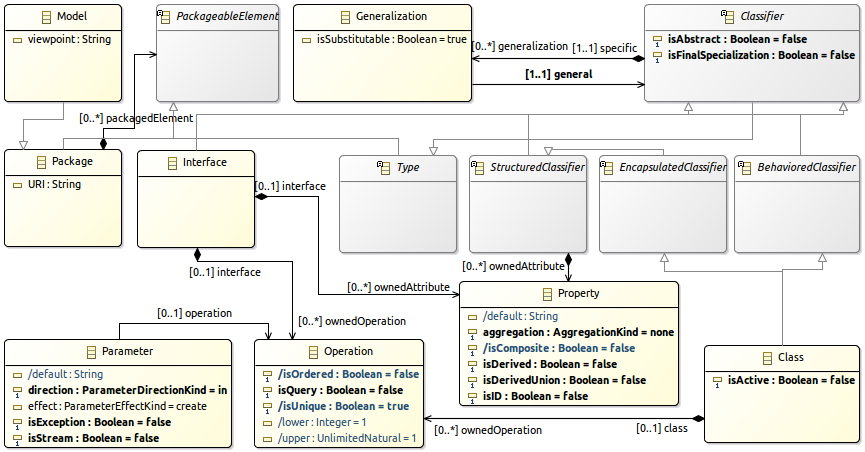
\includegraphics[width=\textwidth]{umlClassDiagramSimple01}
    \end{center}
    \label{fig:uml_metamodel_class}
    \legend{Source: Image created by the author using the \emph{Eclipse IDE}. metamodel from \emph{EMF plug-in}}
\end{figure}

\begin{figure}[H]
    \caption{An example of a model \emph{UMLClassDiagram} visualized in two different ways}
    \centering
	\begin{subfigure}[h]{.35\textwidth}
		\caption{Abstract Syntax}
		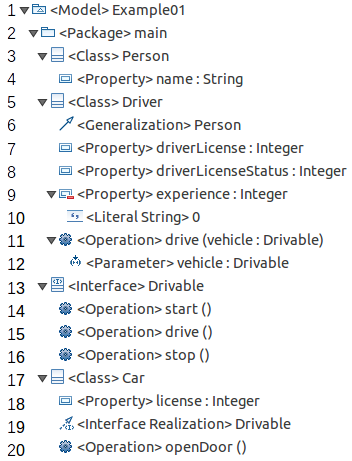
\includegraphics[width=\textwidth]{umlClassDiagramExample01}
	\end{subfigure}
	\begin{subfigure}[h]{.64\textwidth}
		\caption{Concrete Syntax}
		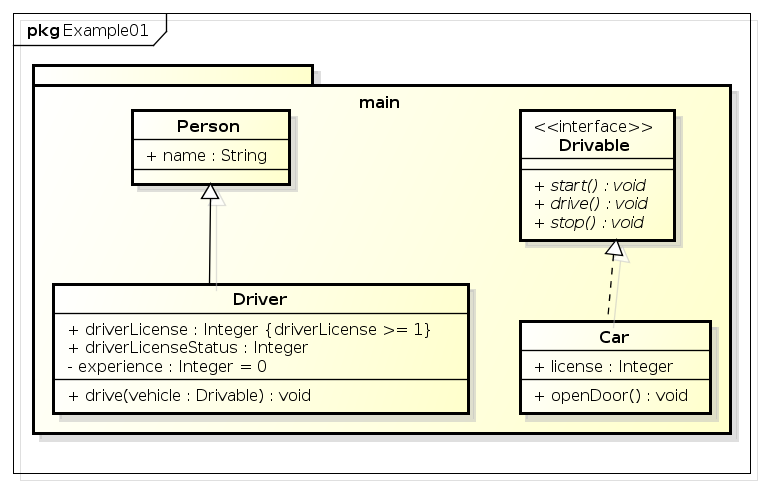
\includegraphics[width=\textwidth]{umlClassDiagramExample01_Diagram}
		\label{fig:uml_metamodel_class_example_concrete}
	\end{subfigure}
    \label{fig:uml_metamodel_class_example}
    \legend{Source: Image created by the author using the \emph{Astah Software}.}
\end{figure}

According to the metamodel, a \emph{Classifier} may have a \emph{Generalization} (i.e. inheritance), illustrated with a straight arrow from \emph{Driver} to \emph{Person} in the example on the Figure \ref{fig:uml_metamodel_class_example_concrete}, or an \emph{InterfaceRealization}  illustrated with a dashed arrow from \emph{Car} to \emph{Drivable}. Moreover, a \emph{Class} is possible to have not only \emph{Properties} (through the aggregation \emph{ownedAttribute}), but also \emph{Operations} (through the \emph{ownedOperation} attribute), which themselves may have \emph{Parameters}. This characteristic is analogous to \emph{Interfaces}. In the running example the \emph{Person} has the \emph{Property name}, as well as the \emph{Driver} has the \emph{Property driverLicense} and the \emph{Operation drive(Drivable):void}. 

%-------------------
% Subsection
%-------------------
\subsection{UML Sequence Diagram}
The \emph{UMLSequenceDiagram} is essentially based on the elements \emph{Interaction}, \emph{Lifeline}, and \emph{Messages}. A simplified view of the metamodel is given on the Figure \ref{fig:uml_metamodel_sequence}. According to \citet[p. 563]{omg2007unified}: \emph{"Interactions [...] are used to get a better grip of an interaction situation"} \citep[p. 563]{omg2007unified}, by being so, the important aspect of sequence diagrams are the exchange of messages between objects (i.e. interaction). Sequence diagrams are quite flexible in regard to its semantics, so developers interpret the exchange of messages in different ways. Nevertheless, they are interpreted in this thesis in a rather simpler manner. An \emph{Interaction} models one scenario, in which an \emph{Operation} of a \emph{Class} is executed, and contains one or more \emph{Lifelines}, that express the life of an instance of a class. A concrete illustration of these elements is to find in the example in the Figure \ref{fig:uml_metamodel_sequence_example_diagram}.

\begin{figure}[H]
    \caption{Simplification of the \emph{UMLSequenceDiagram} metamodel}
    \begin{center}
        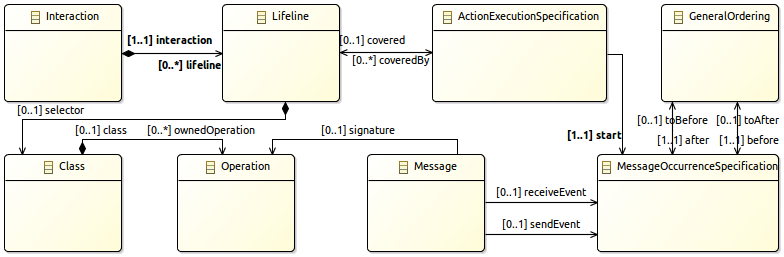
\includegraphics[width=\textwidth]{umlSequenceDiagramSimple01}
    \end{center}
    \label{fig:uml_metamodel_sequence}
    \legend{Source: Image created by the author using the \emph{Eclipse IDE}. metamodel from \emph{EMF plug-in}}
\end{figure}

One \emph{Lifeline} is connected to a \emph{Class} through the attribute \emph{selector} and is \emph{covered by} one \emph{ActionExecutionSpecification}, which in a sequence diagram is depicted by a rectangle over the \emph{Lifeline} and symbolize the time, during which the respective class is executed. An \emph{ActionExecutionSpecification} has then a \emph{MessageOccurenceSpecification} as \emph{start} point, which itself is related to a \emph{Message}. Finally, each \emph{Message} is linked to two \emph{MessageOccurenceSpecifications} $-$ one \emph{receiveEvent} that lies on the beginning and one \emph{sendEvent} that lies on the end of the \emph{Message} $-$ and has a \emph{signature} of an \emph{Operation}. The comprehension of this interpretation over \emph{UMLSequenceDiagrams} requires the reader to grasp the Figure \ref{fig:uml_metamodel_sequence_example} containing one \emph{Interaction} (\emph{Interaction01}), two \emph{Lifelines} (\emph{:Driver} and \emph{:Drivable}), and four \emph{Messages}.

\begin{figure}[H]
    \caption{An example of a model \emph{UMLSequenceDiagram} visualized in two different ways}
    \centering
   	\begin{subfigure}[h]{\textwidth}
   		\caption{Abstract Syntax}
   		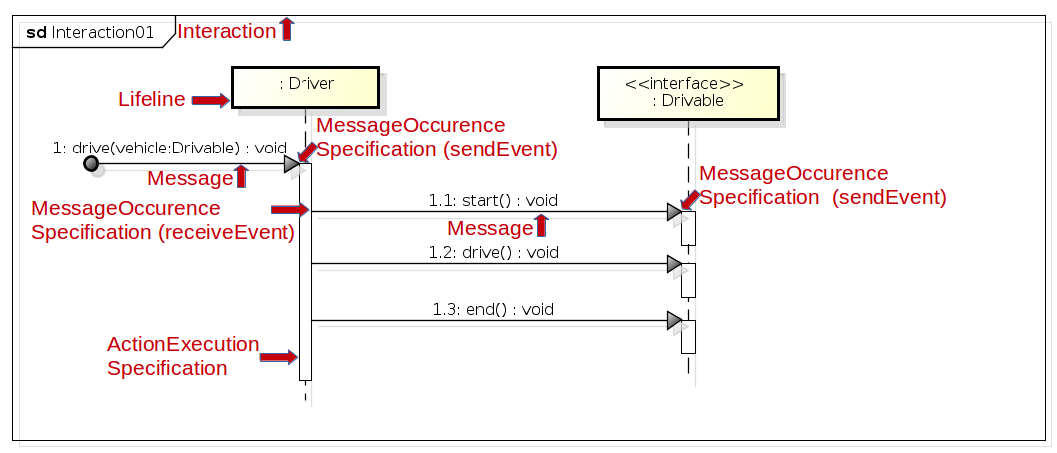
\includegraphics[width=\textwidth]{umlSequenceDiagramExample01}
   	\end{subfigure}
   	\begin{subfigure}[h]{\textwidth}
   		\caption{Concrete Syntax}
   		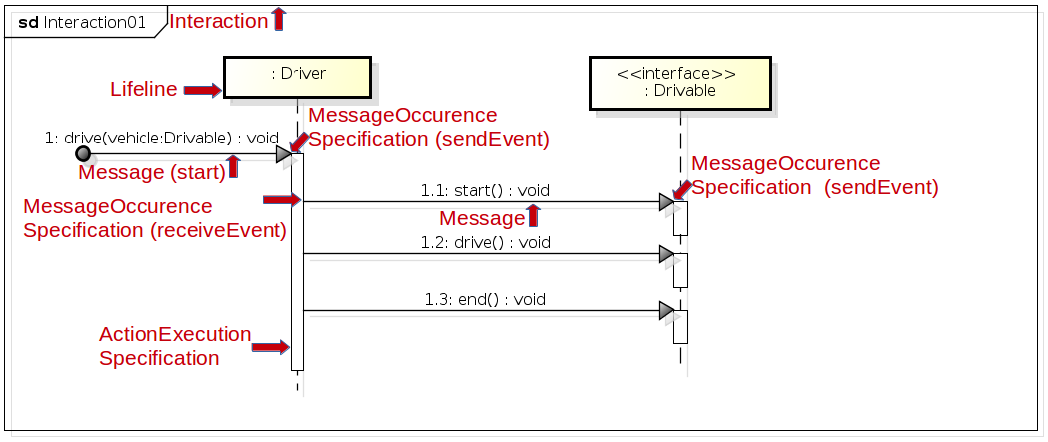
\includegraphics[width=\textwidth]{umlSequenceDiagramExample01_Diagram}
   		\label{fig:uml_metamodel_sequence_example_diagram}
   	\end{subfigure}
    \label{fig:uml_metamodel_sequence_example}
    \legend{Source: Image created by the author using the \emph{Astah Software}.}
\end{figure}

To model the order in which the \emph{Messages} occur, a \emph{GeneralOrdering} establishes an order between two \emph{MessageOccurenceSpecifications}, by signalizing which of them occur \emph{before} or \emph{after} the other. So, in the running example there is a \emph{GeneralOdering} instance holding the \emph{MessageOccurenceSpecifications} related to the \emph{Message 1} as happening \emph{before} the one related to the \emph{Message 1.1} (that is held as \emph{after}).

As stated before, developers tend to interpret and utilize sequence diagrams in different fashions. For this thesis a set of assumptions is made in regard to that. Among them, lifelines represent only classes (excluding thus representation of actors); and only synchronous message are handled.

%-------------------
% Subsection
%-------------------
\subsection{UML Contract}
The \emph{UMLContract} is a slice of the \emph{UML} metamodel, that aims basically to provide constraints to \emph{Operations} and \emph{Properties} of \emph{Classes}. \emph{Operations} may have \emph{pre}, \emph{postconditions}, as well as \emph{Invariants}, which are modeled through the EMF class \emph{Constraint} (on the top of the Figure \ref{fig:uml_metamodel_contracts}).

\begin{figure}[H]
    \caption{Simplification of the \emph{UMLContract} metamodel}
    \begin{center}
        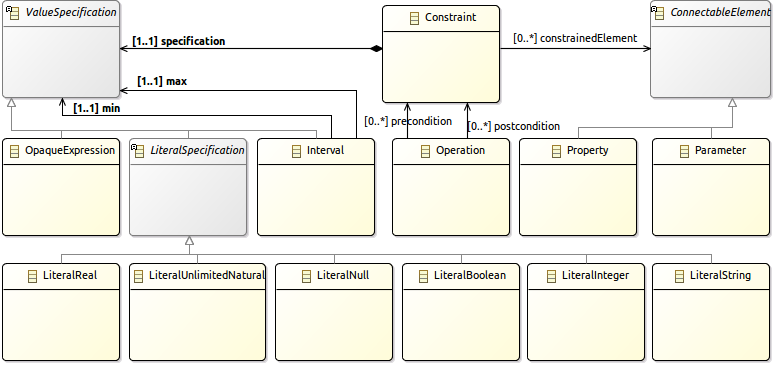
\includegraphics[width=\textwidth]{umlContractSimple01}
    \end{center}
    \label{fig:uml_metamodel_contracts}
    \legend{Source: Image created by the author using the \emph{Eclipse IDE}. metamodel from \emph{EMF plug-in}}
\end{figure}

A \emph{Constraint} may have \emph{constrainedElements}, which in the scope of this thesis are whether \emph{Properties} or \emph{Parameters}. In addition, it has also a \emph{ValueSpecification}, defining the constraint itself, that in this thesis may be a \emph{OpaqueExpression} or an \emph{Interval}. The former is rather a free definition of the constraint composed by a String \emph{body}, and the \emph{language}, in which it is written (see lines 16 to 19 in Figure \ref{fig:uml_metamodel_contracts_example}). The latter defines an interval of values, in which the constrained element has to lie. Therefore, it has one \emph{ValueSpecification} for the minimal and one for the maximal value. Here only \emph{Intervals} with one \emph{LiteralInteger ValueSpecification} for the minimal value will be handled, see an example in the lines 6 to 7 in Figure \ref{fig:uml_metamodel_contracts_example}, that includes elements from \emph{UMLContract}, namely lines 6 to 7 and 14 to 15 (\emph{Constraint} with \emph{Interval}), and lines 16 to 19 (\emph{Constraint} with \emph{OpaqueExpression}).

\begin{figure}[H]
    \caption{The expanded version of the model from the picture \ref{fig:uml_metamodel_class_example} as an example for \emph{UMLContract}. Only abstract syntax is used for this example.}
    \begin{center}
        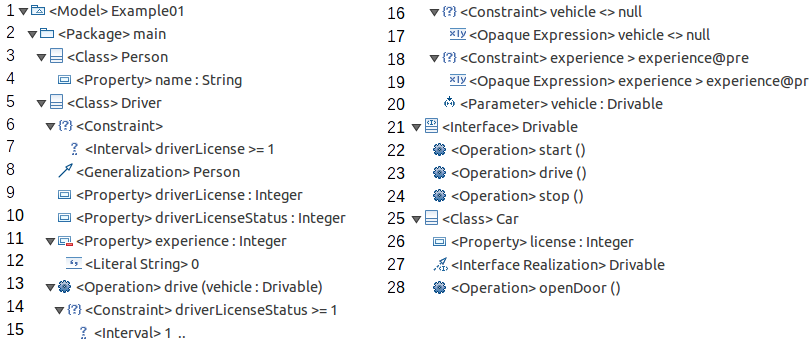
\includegraphics[width=.8\textwidth]{umlContractDiagramExample01}
    \end{center}
    \label{fig:uml_metamodel_contracts_example}
    \legend{Source: Image created by the author using the \emph{Eclipse IDE}.}
\end{figure}

%-------------------
% Subsection
%-------------------
\subsection{Java}
A \emph{Java} model is usually the main artifact of a network of models, in that it comprises much information (both structural and behavioral) about the system under study. It can be visualized either as the digram in the Figure \ref{fig:java_metamodel_example} or as plain-text (Figure \ref{fig:java_metamodel_example_text01}). The first option is used here, since it seems to be more suitable when handling the model for synchronization than a plain-text source-code format. Nevertheless, there are techniques\footnote{https://eclipse.org/modeling/m2t} to transform one format into another.

A new metamodel for \emph{Java} is designed in regard to the necessities of this work and includes not only structural elements (e.g. \emph{Packages}, \emph{Classes}, \emph{Fields}, etc.), but also some behavioral aspects (e.g. \emph{Statements}), the latter are very shallowly modeled here, but could be further developed in future works. Other possibilities for the metamodel included the metamodel\footnote{http://www.eclipse.org/modeling/emf/downloads} provided by the \emph{Eclipse IDE}, whose simplicity hindered its use; or yet the one found in \citet{heidenreich2010closing}, but this one happens to be so extensive that could bring unnecessary complexity to this thesis. The Figure \ref{fig:java_metamodel} reports the whole \emph{Java} metamodel created. Elements in blue are \emph{EMF Ecore} abstract elements, whilst elements in yellow are concrete.

\begin{figure}[H]
    \caption{The Java metamodel created}
    \begin{center}
        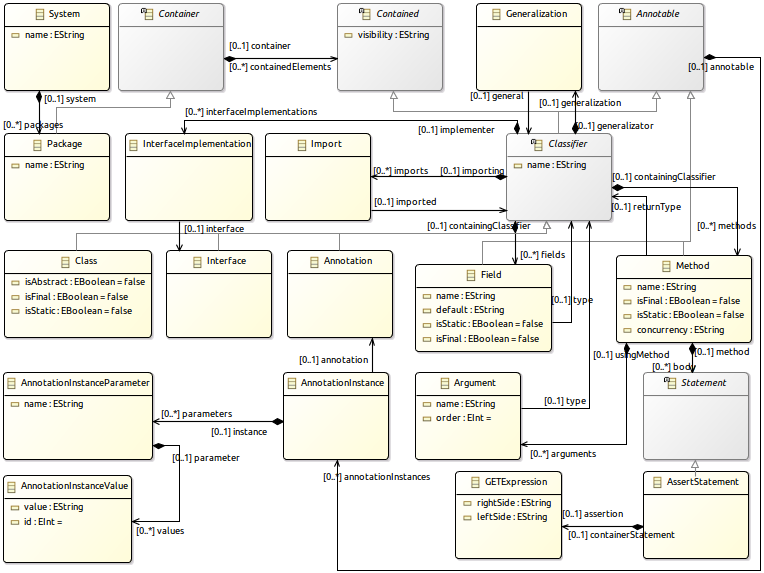
\includegraphics[width=\textwidth]{javaMetamodel}
    \end{center}
    \label{fig:java_metamodel}
    \legend{Source: Image created by the author using the \emph{Eclipse IDE}.}
\end{figure}

The root element is the \emph{System} (on the left top of Figure \ref{fig:java_metamodel}) and represents the whole Java program. It contains \emph{Packages}, that, because of the \emph{Container} inheritance, contains \emph{Classifiers} (through the \emph{Contained} inheritance). The example on the Figure \ref{fig:java_metamodel_example} illustrates concrete types of \emph{Classifiers} in the lines 3, 5 and 48 (\emph{Class}) and 44 (\emph{Interface}).

One \emph{Classifier} may contain \emph{Fields} (lines 4, 6, 10, 11, 49), \emph{Methods} (lines 12, 28, 31, 33, 35, 37), \emph{Imports} (lines 40 to 43), in addition to \emph{InterfaceImplementations} (line 54) $-$ that refer to one \emph{Interface} $-$ and one \emph{Generalization} (line 39), also known as inheritance or extension, which refers to another \emph{Classifier} as its \emph{general}.

A \emph{Method} may have zero or more \emph{Arguments} picture $-$ also known as parameters $-$ likewise \emph{Statements} (to find on the left bottom of the Figure \ref{fig:java_metamodel}). In this imperative perspective of the \emph{Java} metamodel, each method has thus an ordered list of \emph{Statements}, representing usually commands that carve the behavior of the program. In a full representation of the \emph{Java} metamodel, they could be of several kinds (e.g. arithmetic expression, logic expression, method call, control structure like \emph{if}), but for the scope of this bachelor thesis only \emph{AssertStatements} are modeled. An \emph{AssertStatement} basically tests a logical expression. If it does not hold, than an exception is thrown. The only logical expression supported here is the \emph{greater-or-equal expression} (\emph{GETExpression}, left bottom on the Figure \ref{fig:java_metamodel}), but again the construction of a more complete metamodel shall be possible in a wider scope. An example of a \emph{Method} with \emph{AssertStatement} is to find on the lines 28 to 30 and 33 to 36 of the Figure \ref{fig:java_metamodel_example}.

\begin{figure}[H]
    \caption{The equivalent \emph{Java} version of the \emph{UML} models from the Figures \ref{fig:uml_metamodel_class_example},  \ref{fig:uml_metamodel_contracts_example} and \ref{fig:uml_metamodel_sequence_example} in abstract syntax.}
    \begin{center}
        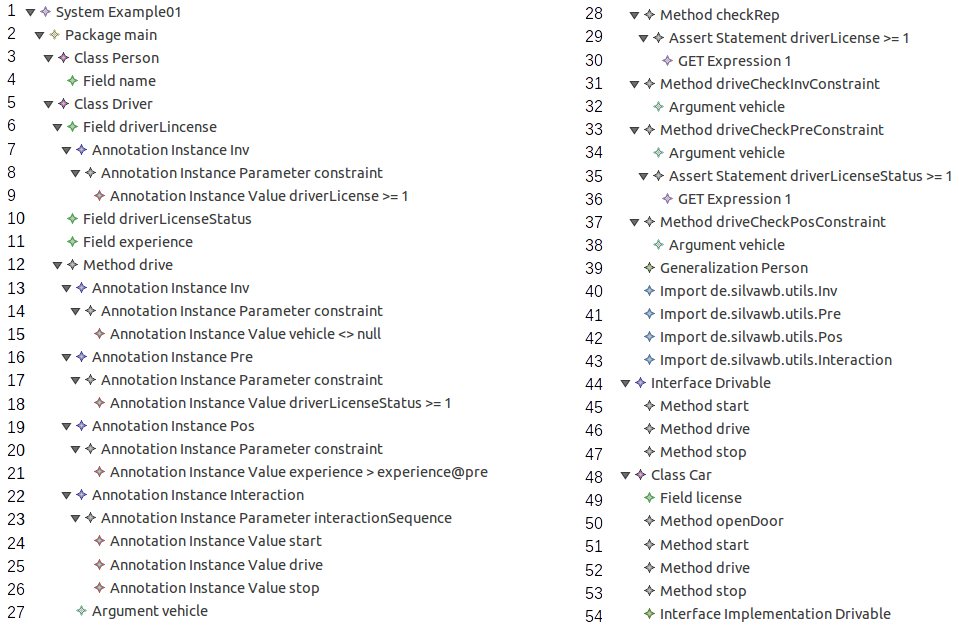
\includegraphics[width=\textwidth]{javaMetamodelExample01}
    \end{center}
    \label{fig:java_metamodel_example}
    \legend{Source: Image created by the author using the \emph{Eclipse IDE}.}
\end{figure}

To finish the description of the metamodel, there is the \emph{Annotation}, which is also a kind of \emph{Classifier}. An \emph{AnnotationInstance} is then contained by an \emph{Annotable} element (i.e \emph{Classifier}, \emph{Field}, or \emph{Method}) and may contain \emph{AnnotationInstanceParameters}, which themselves may contain \emph{AnnotationInstanceValues}. The Figure \ref{fig:java_metamodel_example} contains examples of annotations on the lines 7 to 9 and 13 to 26.

The figure \ref{fig:java_metamodel_example_text01} shows the plain-text view over the \emph{class} \emph{Driver} of the previous example model only with some small differences. In fact, this plain-text view has two elements that are not modeled in our \emph{Java} metamodel, namely expansion of logical expressions (line 21) and method calls (lines 36 to 46), but anyway it exposes the ideas behind the use of \emph{Annotations} (lines 9 and 29 to 34) and their relation with \emph{UMLSequenceDiagrams} and \emph{UMLContracts}. More details are shown in the next chapter.

\begin{figure}[H]
    \caption{A more comprehensive \emph{Java} model based on the Figure \ref{fig:java_metamodel_example}, but depicted in plain-text form, expressing the Java concrete syntax.}
    \begin{center}
        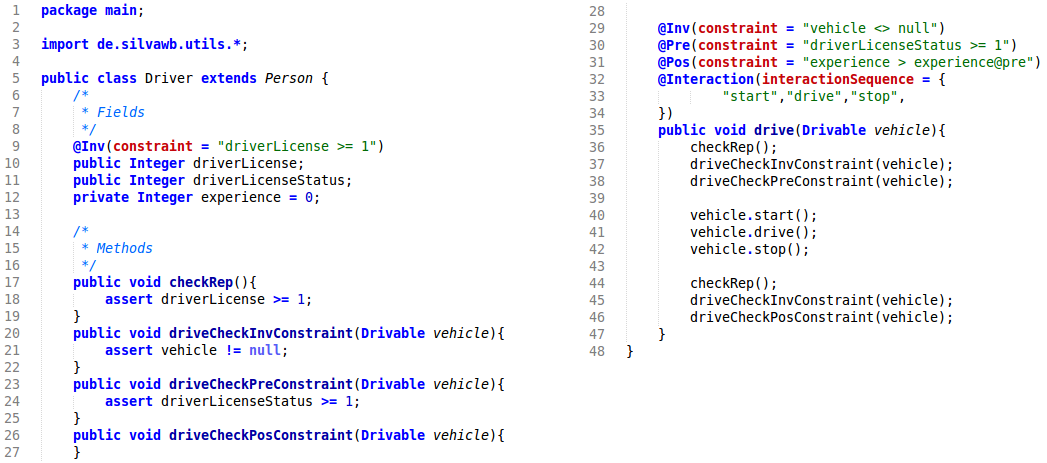
\includegraphics[width=\textwidth]{javaMetamodelExample01_Text}
    \end{center}
    \label{fig:java_metamodel_example_text01}
    \legend{Source: The Author.}
\end{figure}

%---------------------------------------------
% Section
%---------------------------------------------
\section{Metamodel Relations}
\label{subsec:MetamodelRelations}
With all the metamodels defined, the definition of the relations between their elements can be done. In order to accomplish that, TGG is used to code the relations, because it has been extensively used in current academic research and because it is supported by several tools for synchronization. Other options included the \emph{ATL} \citep{jouault2008atl}, which does not seem to be enough ripe for our use; or the \emph{Henshin} \citep{arendt2010henshin}, that is not widely supported for the best synchronization tools \citep{hildebrandt2013survey}. A theoretical basis of TGG has been given in Chapter \ref{ch:foundations}. Here the most representative relations are presented, as well as some explanations over them. The complete version of the TGG's are attached to this thesis in digital form.

%-------------------
% Subsection
%-------------------
\subsection{Relations between \emph{UMLClassDiagram} and \emph{Java}}
\label{subsec:umlClassDiagram2Java}
Figure \ref{fig:umlClassDiagram2java_type} shows the triple type graph for the relations between the \emph{UMLClassDiagram} (left) and the \emph{Java} (right) domains, with the correspondence domain being in the middle. In this graph, elements from the left domain are connected to the elements on the right domain, with whom they have a relation. So, the element \emph{Model} in \emph{UMLClassDiagram} has a relation to the element \emph{System} in \emph{Java}; analogously, a \emph{Property} in \emph{UMLClassDiagram} is related to an \emph{Field} in \emph{Java}, namely whenever the former is created, the correspondent latter has to be created according to the former's characteristics (i.e. name, type, the class it belongs, etc.).

\begin{figure}[H]
    \caption{The triple type graph for \emph{UMLClassDiagram} and \emph{Java}}
    \begin{center}
        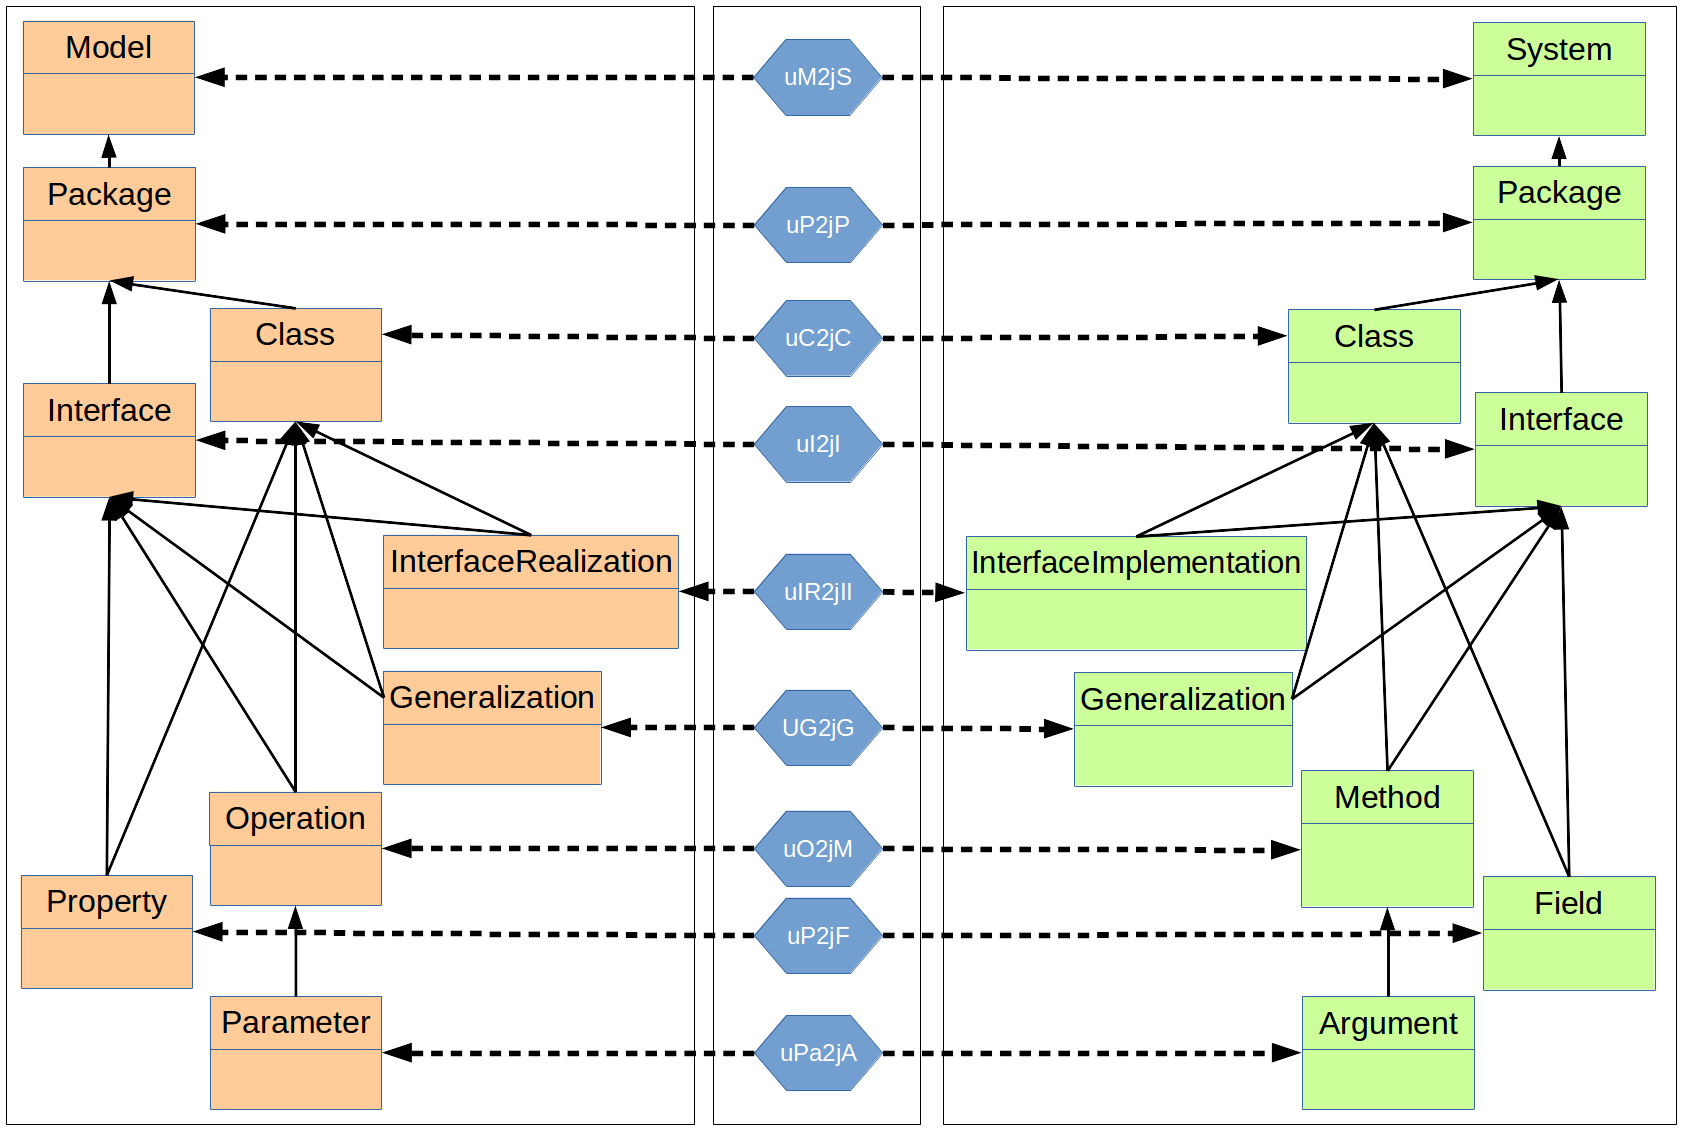
\includegraphics[width=.7\textwidth]{umlClassDiagram2java_type}
    \end{center}
    \label{fig:umlClassDiagram2java_type}
    \legend{Source: The author}
\end{figure}

The triple rules describing the relation between \emph{Model} and \emph{System}, as well as \emph{Package} (UML) and \emph{Package} (Java) is available on Figure \ref{fig:tgg_rule}. The triple rule encoding the relation between an \emph{Attribute} of a \emph{Class} in \emph{UMLClassDiagram} and a \emph{Field} of a \emph{Class} in \emph{Java} is shown on the Figure \ref{fig:uCAttribute2jCField}. In essence, this rule formalizes the fact that for every \emph{Class Attribute} (white filling object in the image) in \emph{UMLClassDiagram} a correspondent \emph{Class Field} in \emph{Java} is supposed to exist with corresponding values for the respective meta-attributes. These are \emph{name}, \emph{default}, \emph{isStatic}, \emph{isLeaf}, and \emph{visibility} in the \emph{UML Property}, which correspond respectively to \emph{name}, \emph{default}, \emph{isStatic}, \emph{isFinal}, and \emph{visibility} in the \emph{Java Field}.

\begin{figure}[H]
    \caption{The triple rule \emph{uClassAttribute2jClassField}}
    \begin{center}
       	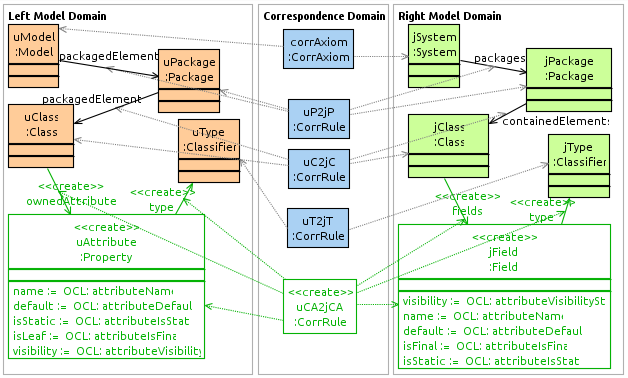
\includegraphics[width=.7\textwidth]{uCAttribute2jCField}
    \end{center}
    \label{fig:uCAttribute2jCField}
    \legend{Source: Image created by the author using the \emph{Eclipse IDE}.}
\end{figure}

\begin{figure}[H]
    \caption{The triple rule \emph{uInterfaceRealization2jInterfaceImplementation}}
    \begin{center}
       	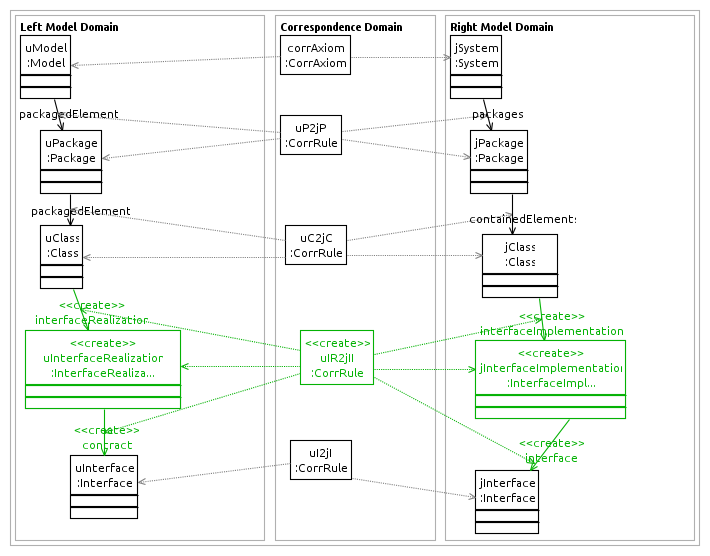
\includegraphics[width=.7\textwidth]{uIRealization2jIImplementation}
    \end{center}
    \label{fig:uIRealization2jIImplementation}
    \legend{Source: Image created by the author using the \emph{Eclipse IDE}.}
\end{figure}

Analogously, the figure \ref{fig:uIRealization2jIImplementation} shows the triple rule $L_sL_cL_t \rightarrow R_sR_cR_t$ for \emph{UML InterfaceRealization} and \emph{Java InterfaceImplementation}. In this case, an \emph{InterfaceRealizations} have none meta-attributes to be described, besides the associations with \emph{Class} and \emph{Interface}. This rule could be read as follows: Given a state $S_i$ with a triple graph $L_sL_cL_t$ (LHS) containing all the color-filled elements of Figure \ref{fig:uIRealization2jIImplementation}, the creation of a \emph{UML InterfaceRealization} ($uInterfaceRealization \in R_s$) implies the creation of a \emph{Java InterfaceImplementation} ($uInterfaceImplementation \in R_t$) connected by an element of the correspondence domain ($uIR2jII \in R_c$) and vice-versa.

%-------------------
% Subsection
%-------------------
\subsection{Relations between \emph{UMLSequenceDiagram} and \emph{Java}}
\label{subsec:UmlSequenceDiagram2Java}
Figure \ref{fig:umlSequenceDiagram2java_type} shows the triple type graph for the relations between the \emph{UMLSequenceDiagram} (left) and the \emph{Java} (right) domains, with the correspondence domain being in the middle. A \emph{Lifeline} and its respective \emph{ActionExecutionSpecification} are related to an \emph{AnnotationInstance} and its respective \emph{AnnotationInstanceParameter}. So, every \emph{Lifeline} regarding to one specific \emph{Method} is related to one \emph{AnnotationInstance} over this method, responsible for representing in the Java model the sequence of method calls modeled by the sequence diagram. An example of such annotation may be seen in the line 32 of the Figure \ref{fig:java_metamodel_example_text01}. The rule responsible for this relation is depicted in Figure \ref{fig:uILifeline2jMAnnotation}. Briefly, each \emph{Lifeline} (\emph{uLifeline}), together with related elements \emph{uAExecSpecification}, \emph{uMOSSpec} and \emph{uMessage}, is connected to an \emph{AnnotationInstance} (\emph{jAnnInstance}) and a \emph{AnnotationInstanceParameter} (\emph{jAnnInstParam}) belonging to an already existing method (\emph{jMethod}) and referencing an already existing \emph{Annotation} (\emph{InteractionSequenceAnnotation} with name \emph{Interaction}).

\begin{figure}[H]
    \caption{The triple type graph for \emph{UMLSequenceDiagram} and \emph{Java}}
    \begin{center}
        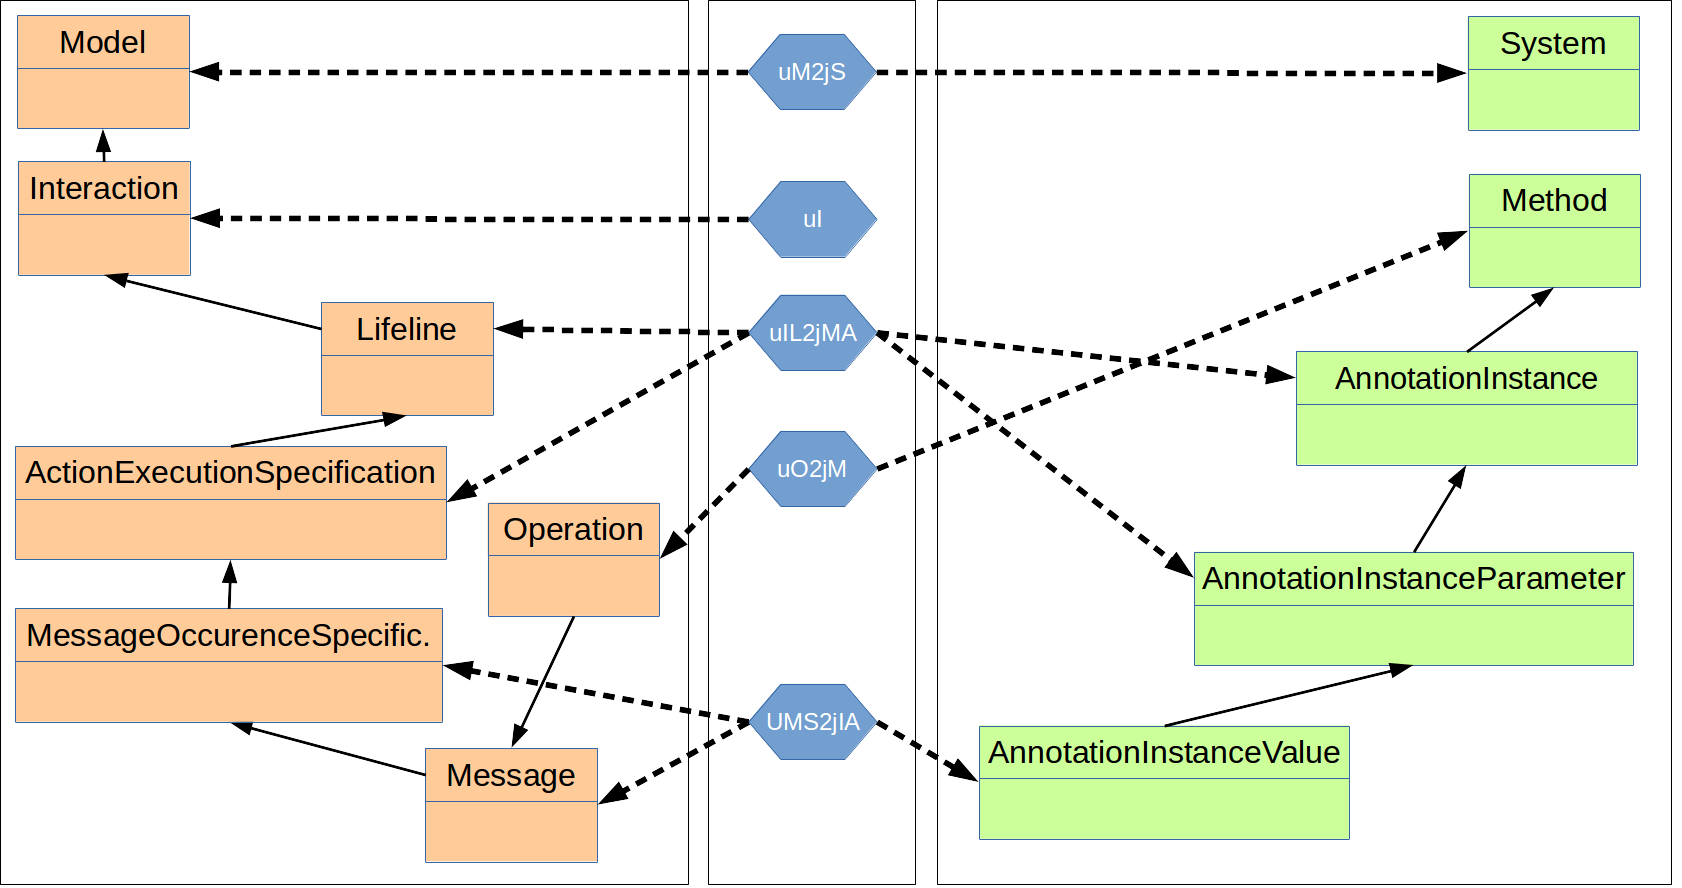
\includegraphics[width=.7\textwidth]{umlSequenceDiagram2java_type}
    \end{center}
    \label{fig:umlSequenceDiagram2java_type}
    \legend{Source: The author}
\end{figure}

Furthermore, for each \emph{MessageOccurenceSpecification} and its respective \emph{Message} (i.e. a method call in the sequence diagram) exists one \emph{AnnotationInstanceValue} containing the name of the invoked method in the Java model (see line 33 of Figure \ref{fig:java_metamodel_example_text01}). In our implementation this is done by two rules. The first rule is in Figure \ref{fig:uMessageSequence2jInteractionAnnotation} and is responsible for the first \emph{MessageOccurenceSpecification} in the \emph{Lifeline} (e.g. the \emph{Message} \emph{1.1: start(): void} in Figure  \ref{fig:uml_metamodel_sequence_example_diagram}). The second rule is in Figure \ref{fig:uMessageSequence2jInteractionAnnotation_2} and is responsible for further \emph{MessageOccurenceSpecifications} in the \emph{Lifeline} (e.g. the \emph{Message} \emph{1.2: drive(): void} or \emph{1.3: stop(): void} in Figure  \ref{fig:uml_metamodel_sequence_example_diagram}). The relation is split, because in the first rule a \emph{GeneralOrdering} (\emph{uOrdering}) links the \emph{start message} (\emph{uStartMessage}) of \emph{uLifeline} to the first \emph{Message} leaving \emph{uLifeline}, whereas in the second rule, \emph{uOrdering} links two ordinary \emph{Messages} leaving \emph{uLifeline}, namely \emph{uMsgBefore} and \emph{uMsgAfter}.

\begin{figure}[H]
    \caption{The triple rule \emph{uLifeline2jMethodAnnotation}}
    \begin{center}
        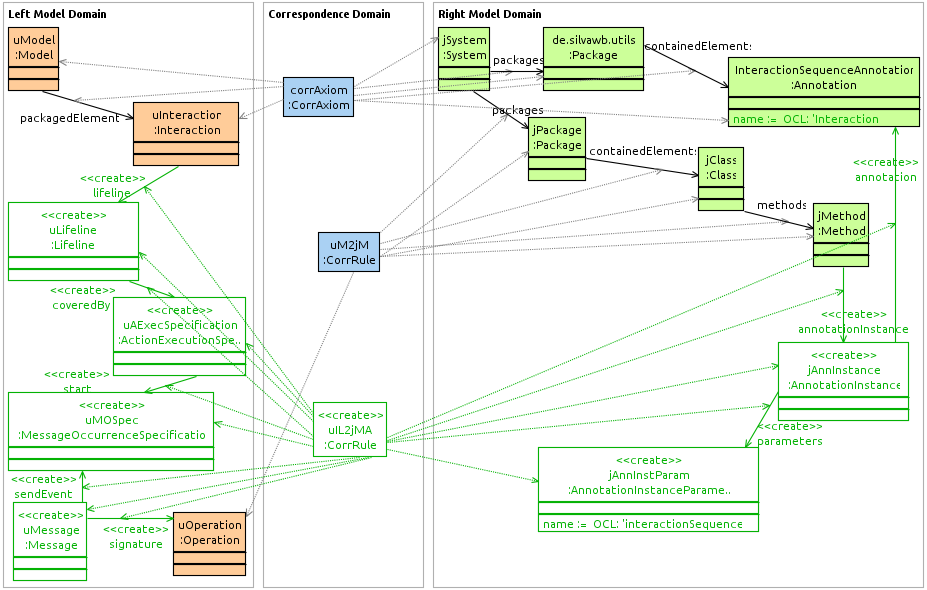
\includegraphics[width=.8\textwidth]{uILifeline2jMAnnotation}
    \end{center}
    \label{fig:uILifeline2jMAnnotation}
    \legend{Source: Image created by the author using the \emph{Eclipse IDE}.}
\end{figure}

The rule \emph{uMessageSequence2jInteractionAnnotation} encodes the fact, that every \emph{Message} (\emph{uMOSAfter}) coming right after the initial \emph{Message} (\emph{uStartMessage}) of \emph{uLifeline} has a correspondent \emph{AnnotationInstanceValue} (\emph{jAnnInstValue}) containing the same \emph{name} as \emph{uOparationAfter}, and being child of a \emph{AnnotationInstanceParameter} (\emph{jAnnInstParam}) with name \emph{interactionSequence}.

%FIXME: Latex: rule name broken
The occurrence order of the \emph{Messages} is handled by the rule \emph{uMessageSequence2jInte-} \emph{ractionAnnotation\_2} through the attribute \emph{id} in the \emph{AnnotationInstanceValue} objects.
More specifically, $jAnnInstValueAfter.id = jAnnInstValueBefore.id + 1$. This field is used in the Java model to indicate the order of the respective objects.

\begin{figure}[H]
    \caption{The triple rule \emph{uMessageSequence2jInteractionAnnotation}}
    \begin{center}
        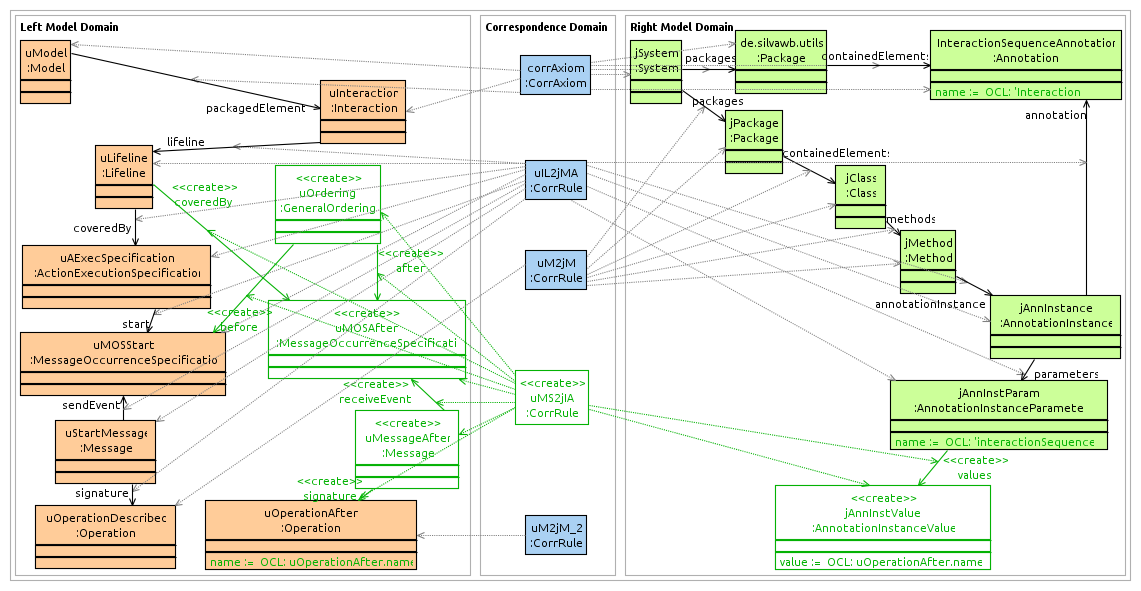
\includegraphics[width=.9\textwidth]{uMessageSequence2jInteractionAnnotation}
    \end{center}
    \label{fig:uMessageSequence2jInteractionAnnotation}
    \legend{Source: Image created by the author using the \emph{Eclipse IDE}.}
\end{figure}

\begin{figure}[H]
    \caption{The triple rule \emph{uMessageSequence2jInteractionAnnotation\_2}}
    \begin{center}
        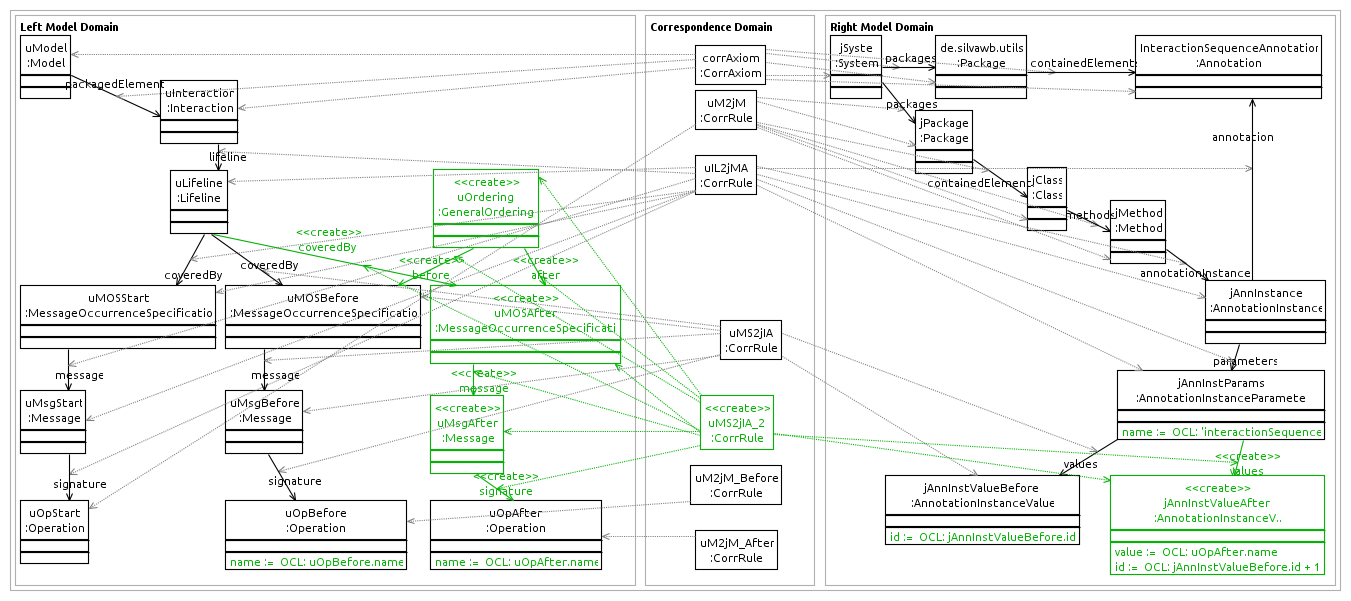
\includegraphics[width=.9\textwidth]{uMessageSequence2jInteractionAnnotation_2}
    \end{center}
    \label{fig:uMessageSequence2jInteractionAnnotation_2}
    \legend{Source: Image created by the author using the \emph{Eclipse IDE}.}
\end{figure}


%-------------------
% Subsection
%-------------------
\subsection{Relations between \emph{UMLContract} and \emph{Java}}
\label{subsec:UmlContracts2Java}

Figure \ref{fig:umlContract2java_type} shows the triple type graph for the relations between the \emph{UMLContract} (left) and the \emph{Java} (right) domains, with the correspondence domain being in the middle. Here a \emph{Constraint} may refer to whether a \emph{Property}, an \emph{Operation} or a \emph{Parameter} and may contain (1) an \emph{OpaqueExpression} or (2) an \emph{Interval}. In the first case both the \emph{Constraint} and \emph{OpaqueExpression} objects are connected to an \emph{AnnotationInstance}, an \emph{AnnotationInstanceParameter}, and an \emph{AnnotationInstanceValue}. Examples of \emph{OpaqueConstraints} are shown in the lines 29 and 31 of the Figure \ref{fig:java_metamodel_example_text01}. The triple rule for the case of a \emph{OpaqueConstraint} over a \emph{Property} is presented in Figure \ref{fig:uCInv2jCInv}. This rule, basically, formalizes that every \emph{OpaqueExpression} (\emph{uOpaqueSpecification}) specifying a \emph{Constraint} (\emph{uConstraint}), which itself constraints a \emph{Property} (\emph{uAttribute}), has an \emph{AnnotationInstanceValue} (containing the same specification as \emph{uOpaqueSpecification}), an \emph{AnnotationInstanceParameter}, and an \emph{AnnotationInstance}, which itself belongs to the \emph{Field} \emph{jField} related to the respective constrained \emph{uAttribute} and references the already existing \emph{Annotation} \emph{Inv} with name \emph{Inv}.

\begin{figure}[H]
    \caption{The triple type graph for \emph{UMLContract} and \emph{Java}}
    \begin{center}
        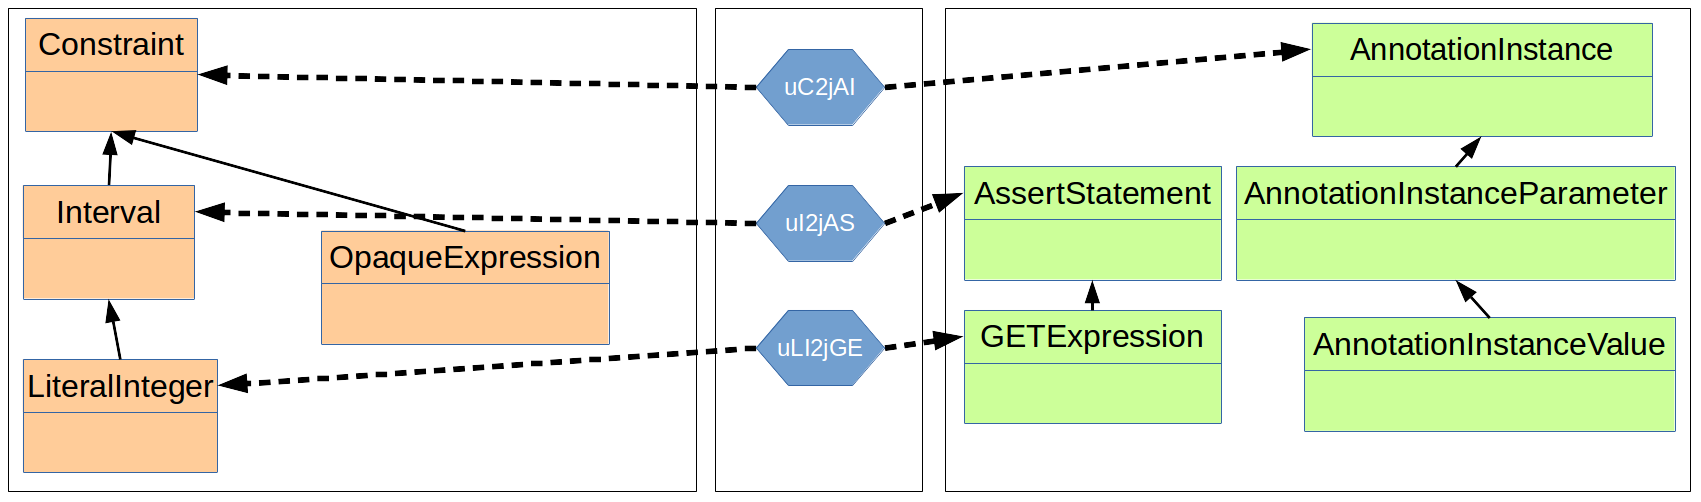
\includegraphics[width=.7\textwidth]{umlContract2java_type}
    \end{center}
    \label{fig:umlContract2java_type}
    \legend{Source: The author}
\end{figure}

The triple rule for the case of an \emph{IntervalConstraint} over a \emph{Parameter} is presented in Figure \ref{fig:uOPPreInt2jMAPreAssert}. The difference to the previous figure, is that now on the source domain, an \emph{Interval} (\emph{uInterval}) is used to specify \emph{uConstraint}, which is a \emph{precondition} to \emph{uOperation} and has a \emph{LiteralInteger} (\emph{uLiteralInt}) as minimal value. Moreover, the creation of these elements create not only \emph{Annotation} elements in the Java model, instead it creates also \emph{AssertStatements} in the form of \emph{GETExpressions} belonging to a previously created \emph{check Method}. 

In our implementation, every \emph{Method} of the Java model has three \emph{check Methods}, namely \emph{checkPreConstraint}, \emph{checkPosConstraint}, and \emph{checkInvConstraint}. By being so, the rule \emph{uOPPreInt2jMAPreAssert} is able to transform \emph{UML interval pre-conditions} into \emph{Java GETExpression}, by using the attribute \emph{uConstrained.name} as left side and the \emph{uLiteralInt.value} as right side of the target expression \emph{jGETExpression}.

\begin{figure}[H]
    \caption{The triple rule \emph{uCInv2jCInv}}
    \begin{center}
        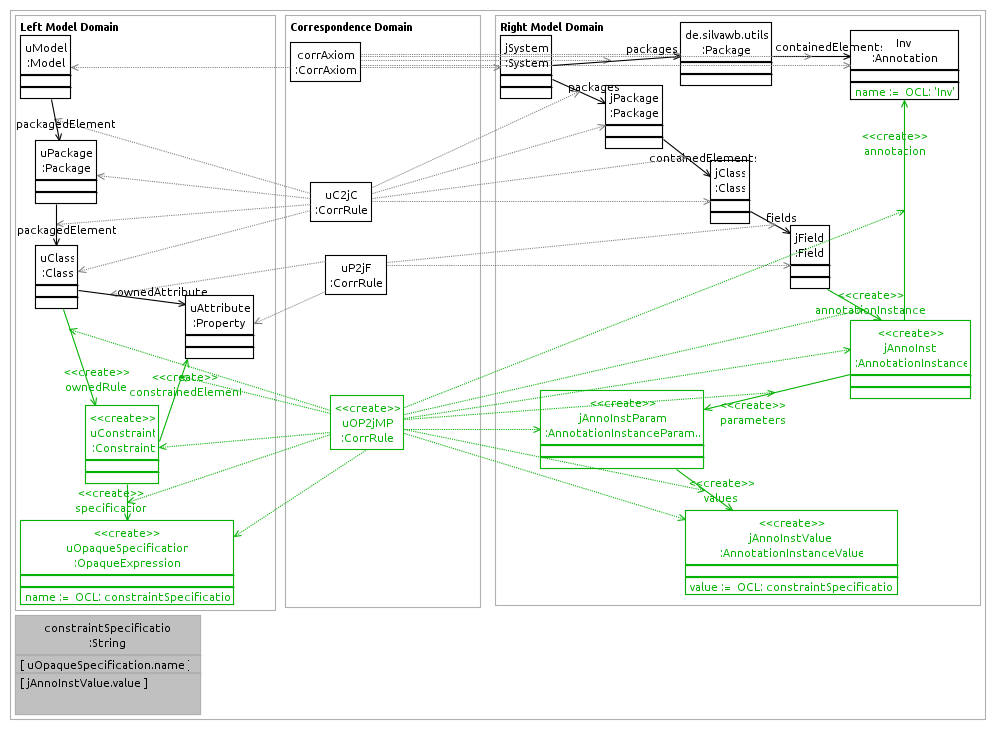
\includegraphics[width=.9\textwidth]{uCInv2jCInv}
    \end{center}
    \label{fig:uCInv2jCInv}
    \legend{Source: Image created by the author using the \emph{Eclipse IDE}.}
\end{figure}
\begin{figure}[H]
    \caption{The triple rule \emph{uOPPreInt2jMAPreAssert}}
    \begin{center}
        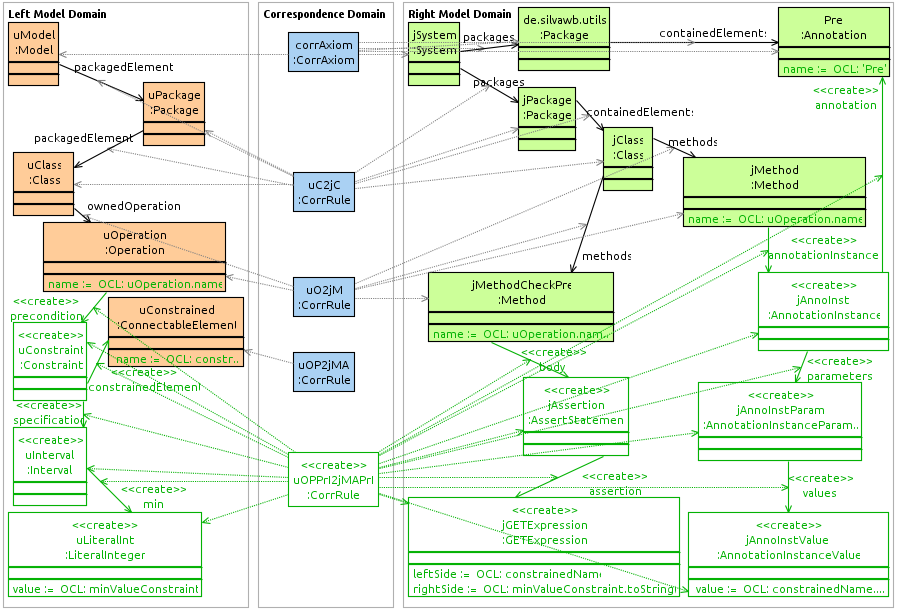
\includegraphics[width=.9\textwidth]{uOPPreInt2jMAPreAssert}
    \end{center}
    \label{fig:uOPPreInt2jMAPreAssert}
    \legend{Source: Image created by the author using the \emph{Eclipse IDE}.}
\end{figure}

%---------------------------------------------
% Section
%---------------------------------------------
\section{Evaluation}
\label{subsec:Evaluation}

%FIXME: Manual breaklines
The three TGG's developed in this thesis have been tested separately through some example scenarios of forward transformation. This means, synchronization is not applied in this evaluation, instead only forward transformations using the three developed TGG's (\emph{umlClassDiagram2java}, \emph{umlSequenceDiagram2java}, \emph{umlContracts2java}) are executed for some example cases, some of them are shown in this section. The Figure \ref{fig:umlClassDiagram2java_Example01} shows the result of a forward transformation from \emph{UMLClassDiagram} to \emph{Java} executed by the \emph{MoTE transformation tool} based on the \emph{umlClassDiagram2java} TGG. This TGG includes the rules presented above (\emph{uClassAttribute2jClassField}, \emph{uInterfaceRealization2jInterfaceImplementation}) plus the following rules, all comprised in digital form, attached to this thesis: \emph{uModel2jSystem} (Axiom), \emph{uPackage2jPackage}, \emph{uClass2jClass}, \emph{uClassOperation2jClassMethod}, \emph{uInterface2jInterface}, \emph{uInterfaceAttribute2jInterfaceField}, \emph{uInterfaceOperation2jInterfaceMethod} and \emph{uCGeneralization- 2jCGeneralization}. In the example, \emph{uModel2jSystem} is applied in line 1; \emph{uPackage2jPackage} in line 2; \emph{uInterface2jInterface} in line 3; \emph{uInterfaceOperation2jInterfaceMethod} in line 4, 5 and 6; \emph{uClass2jClass} in line 7; \emph{uClassAttribute2jClassField} in line 8;  \emph{uInterfaceRealization2jInterface- Implementation} in line 9; and \emph{uClassOperation2jClassMethod} in line 10.

\begin{figure}[H]
    \caption{Example of forward synchronization from a \emph{UMLClassDiagram} model (left) and a \emph{Java} (right) model}
    \begin{center}
       	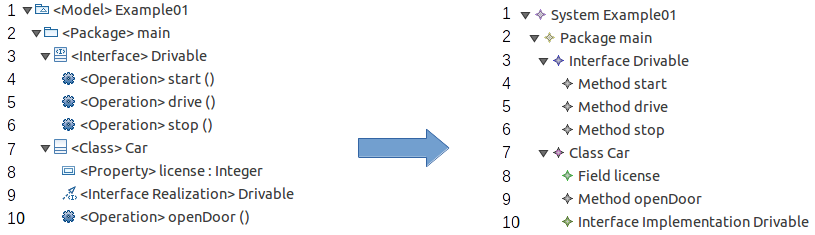
\includegraphics[width=.9\textwidth]{umlClassDiagram2java_Example01}
    \end{center}
    \label{fig:umlClassDiagram2java_Example01}
    \legend{Source: Image created by the author using the \emph{Eclipse IDE}.}
\end{figure}

The problem with the \emph{umlClassDiagram2java} TGG is that it does not encode the fact that the implementing class \emph{Car} should contain the $3$ methods defined by the interface \emph{Drivable} in Java. A possible solution would be the creation of a new rule including an object (\emph{uMethod}) contained by (\emph{uInterface}) in $L_s$ (LHS) linked with the respective \emph{jMethod} contained in \emph{jClass} in $R_t$ (RHS). This new rule should then be evaluated $m$ times by the transformation engine (for the creation of the $m$ methods in \emph{jClass}), but in fact it can be executed only once in the operational semantic scheme proposed by \citet[p. 9]{giese2010toward}. In the same scheme, the creation of such rule would entail a critical pair, given that two different rules have the object \emph{uInterfaceRealization} in the $R_s$. A definite solution is not know by us, therefore this synchronization task ends up being left to the developer. Moreover, \emph{umlClassDiagram2java} is not complete, as it (1) does not comprise a rule for the \emph{Parameter} element of the UML metamodel $-$ By being so, a \emph{Method} would not have its \emph{Parameters} synchronized $-$ and (2) nested \emph{Packages} are not supported.

%FIXME: Manual breaklines
Figure \ref{fig:umlSequenceDiagram2java_Example01} shows the result of a forward transformation from \emph{UMLSequenceDiagram} to \emph{Java} based on the \emph{umlSequenceDiagram2java} TGG, which comprises the rules shown above (\emph{uLifeline2jMethodAnnotation}, \emph{uMessageSequence2jInteractionAnnotation}, \emph{uMessageSequen- ce2jInteractionAnnotation\_2}) plus an axiom \emph{umlInteraction2javaAxiom} responsible for linking an \emph{Interaction} object in UML to an \emph{Annotation} object in Java. In the example, the axiom is used in the lines 1 and 2 of the left and 1, 2, 3 and 4 of the right model; \emph{uLifeline2jMethodAnnotation} is applied for the lines 6, 8, 9 and 19 of the left model, and 8 and 9 of the right model;  \emph{uMessageSequence2jInteractionAnnotation} is applied for the lines 3, 11, 20 of the left, and 10 of the right model; finally, \emph{uMessageSequence2jInteractionAnnotation\_2} is applied once for the lines 4, 14 and 21 of the left, and 11 of the right model; and once more for the lines 5, 17 and 22 of the left, and 12 of the right model. The rest of the elements, like the \emph{Package main}, the \emph{Class Driver} and the \emph{Operations} are handled by extra rules based on the \emph{umlClassDiagram2java} TGG. This is made, in order to build this richer scenario. Observe that, in a real world synchronization situation these extra rules would not be necessary, once the respective elements would have been created by the \emph{umlClassDiagram2java}.

\begin{figure}[h]
    \caption{Example of forward synchronization from a \emph{UMLSequenceDiagram} model (left) and a \emph{Java} (right) model}
    \begin{center}
       	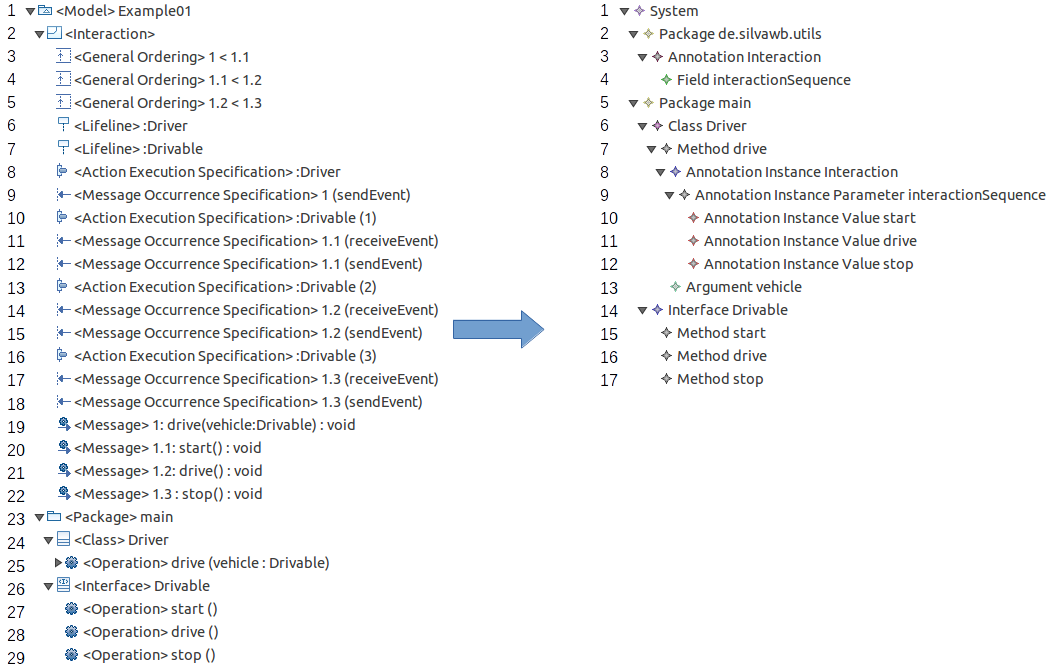
\includegraphics[width=\textwidth]{umlSequenceDiagram2java_Example01}
    \end{center}
    \label{fig:umlSequenceDiagram2java_Example01}
    \legend{Source: Image created by the author using the \emph{Eclipse IDE}.}
\end{figure}

This TGG makes several assumptions that narrow the possibilities of sequence diagrams. In general, only simple synchronous messages are supported, so create, delete or reply messages are not supported; actor, entity or other types of lifelines cannot occur; furthermore, it is supposed, that further features like \emph{InteractionUse} or \emph{CombinedFragment} (see \citep[p. 621 and p. 630]{omg2015meta}) also do not happen in the sequence diagrams. In a broader view, one could say, that the rule is too simple, once it captures basically only the order of the message occurrences and transforms it into annotations in the Java model (and vice-versa). Indeed, it exposes the problem of TGG's to deal with non MOF-appropriate models, since that more powerful tools to handle method calls inside a Java method would be desired to build a more comprehensive transformation from sequence diagrams to Java, for instance. Nevertheless, for the simplified scenario of this thesis the implemented TGG seems to work properly. A transformation rule that encodes the order of elements in the left and right domain were not known by us to exist in the current literature, so in this sense this feature is novel and contributive.

%FIXME: Manual breaklines
Figure \ref{fig:umlContracts2java_Example01} shows the result of a forward transformation from \emph{UMLContract} to \emph{Java} using the \emph{umlContract2java} TGG. Beyond the two rules exposed in the previous section (\emph{uCInv2- jCInv}, \emph{uOPPreInt2jMAPreAssert}), this TGG comprises basically one Axiom; more three rules that encode the relation between \emph{UML Opaque Constraints} and \emph{Java Annotations} (\emph{uOPPre2jM- APre},  \emph{uOPPos2jMAPos}, \emph{uOInv2jMAInv}, respectively for \emph{pre}, \emph{post} and \emph{invariant} constraints); and more two rules that encode the relation between \emph{UML Interval Constraints} and \emph{Java Annotations} plus \emph{Assertions} (\emph{uOPPosInt2jMAPosAssert}, \emph{uCInvInt2jCInvAssert}, respectively for \emph{post} and \emph{invariant constraints}). In the example the axiom is used on the line 1 of the left, and 1 to 5 of the right model and creates constraint \emph{Annotations}; \emph{uCInvInt2jCInvAssert} is used on the lines 4 and 5 of the left, and 9 to 11, as well as 15 to 16 of the right model; \emph{uOPPreInt2jMAPreAssert} is used on the lines 10 and 11 of the left, and 19 to 20, as well as 27 to 29 of the right model;  \emph{uOInv2jMAInv} is used on the lines 12 and 13 of the left, and 30 to 32 of the right model; finally, \emph{uOPPos2jMAPos} is used on the lines 14 and 15 of the left, and 24 to 26 of the right model. The rest of the elements are transformed by other rules, just like in the TGG \emph{umlClassDiagram2java}.

\begin{figure}[H]
    \caption{Example of forward synchronization from a \emph{UMLContract} model (left) and a \emph{Java} (right) model}
    \begin{center}
       	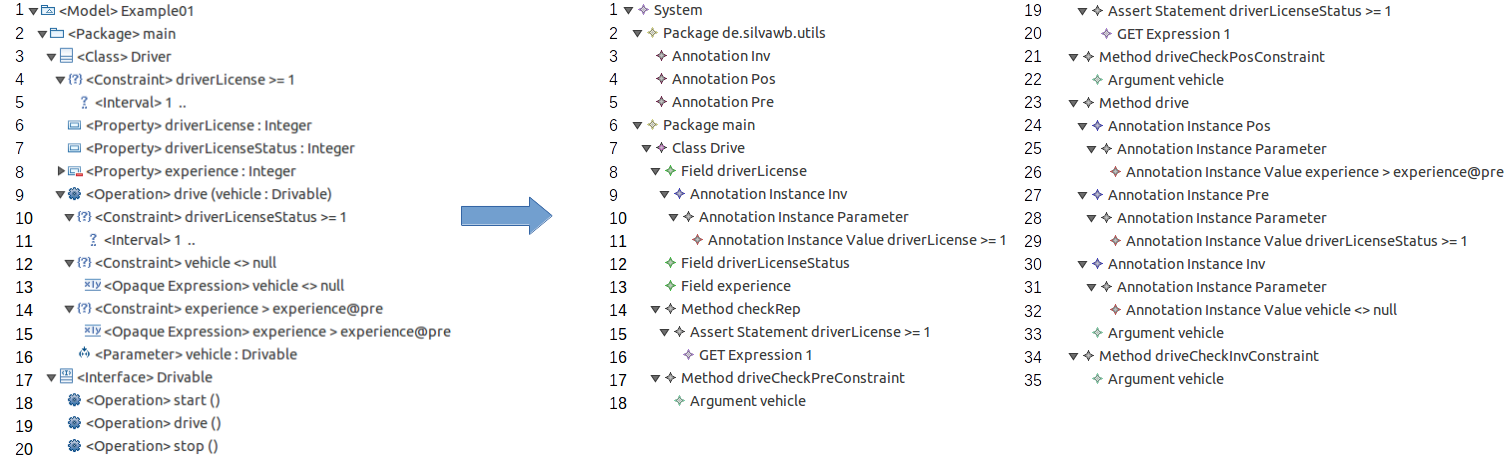
\includegraphics[width=\textwidth]{umlContracts2java_Example01}
    \end{center}
    \label{fig:umlContracts2java_Example01}
    \legend{Source: Image created by the author using the \emph{Eclipse IDE}.}
\end{figure}

This TGG does not seem to present big problems, except that it is not complete, since neither \emph{invariant interval constraints} for methods, nor non-integer \emph{interval constraints} have been developed. Moreover, the implemented rules for \emph{interval constraints} support only \emph{great-or-equal-than expression}. On the other hand, the extension of the current TGG version in direction to completeness seems to be possible, so is the extension in the direction of building unit test cases based on the contracts.

%%%%%%%%%%%%%%%%%%%%%%%%%%%%%%%%%%%%%%%%%%%%%%%%%%%%%%%%%%%%%%%%%%%%%%%%
% Chapter
%%%%%%%%%%%%%%%%%%%%%%%%%%%%%%%%%%%%%%%%%%%%%%%%%%%%%%%%%%%%%%%%%%%%%%%%
\chapter{Synchronization of Models in the Java Technological Space}
\label{chapter:metamodel_synchronization}

In the last chapter the relations between some metamodels of the Java technological space were presented in terms of triple graphs, organized as triple rules and consequently in triple graph grammars. Each TGG was shown in a different section (namely \ref{subsec:umlClassDiagram2Java}, \ref{subsec:UmlSequenceDiagram2Java} and \ref{subsec:UmlContracts2Java}) and represents a different edge of the network of models built (see Figure \ref{fig:network_metamodels}). By being so, each edge corresponds to a different synchronization problem and can be sold, generally speaking, independently from the others. Most of the research in the realm deals with such situation, therefore there are several approaches attempting to solve model synchronization between two models using TGG.

Between them is the \emph{FUJABA} \citep{nickel2000fujaba}, a standalone application that uses TGG to code the relations. Or the \emph{CoWolf}, an extensible framework based on \emph{Eclipse Plug-ins} supporting a pair of metamodels according to \citet{getir2015cowolf}, but that uses \emph{Henshin} \citep{arendt2010henshin} to encode the relations. Finally, there is the \emph{MoTE} transformation tool, a series of \emph{Eclipse Plug-ins} for creating TGG's, both graphically and textually, and for transforming models based on these TGG's. We take \emph{MoTE} for the most adequate option for our needs, mainly because of extensive literature about it (\citep{giese2009efficient} and \citep{hildebrandt2012mdelab}) and the easy integration with other technologies, like the \emph{EMF Ecore} or other useful \emph{Eclipse Plug-ins}.

\begin{figure}[H]
    \caption{Synchronization scheme of the \emph{MoTE} tool}
    \begin{center}
        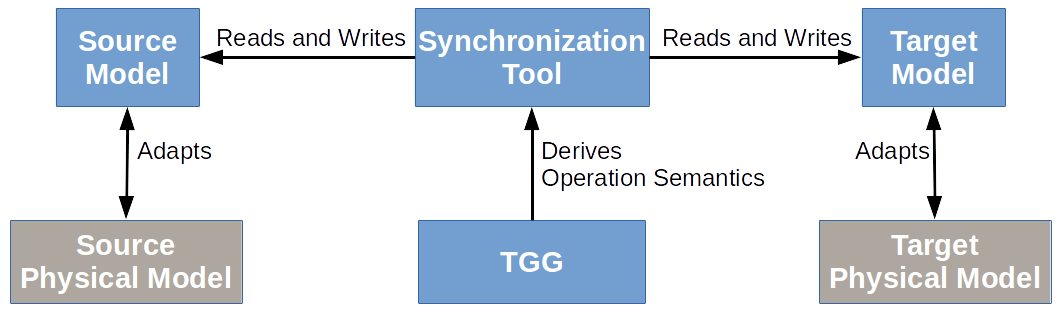
\includegraphics[width=25em]{MoTE_scheme}
    \end{center}
    \label{fig:MoTE_scheme}
    \legend{Source: Adapted from \citep{giese2010model}.}
\end{figure}

The Figure \ref{fig:MoTE_scheme} summarizes how the \emph{MoTE} tool works. Basically, the input TGG is used to derive the operational semantics of the transformation between the source and target models, which are read and written by the synchronization tool. Only these first components (highlighted in the picture) are treated in this thesis, since \emph{MoTE} is used to execute each transformation implemented in Chapter \ref{subsec:MetamodelRelations} (see discussion in Chapter \ref{subsec:Evaluation}). Note, however, that the final practical application of the synchronization is only possible through the adaptation of the logical models (presented so far in form of abstract syntax, e.g Figure \ref{fig:java_metamodel_example}) to physical models (presented so far in form of concrete syntax, e.g Figure \ref{fig:java_metamodel_example_text01}). Such situation is out of the scope of this thesis. 

As stated before, there exists one instance of the synchronization scheme in Figure \ref{fig:MoTE_scheme} for each edge of our network of models. But as the whole network have to be maintained, it raises the problem of synchronizing not only two models separately, but instead a whole set of models. In this scenario, each modification on a specific model has to be propagated through the net. For that, a theoretical analysis of the problem followed by an algorithm is presented below. The goal of this chapter is not the definition of the synchronization algorithm or the implementation of a tool such as \emph{MoTE}, but the definition of an algorithm for the synchronization of a whole network of models that uses an already proposed synchronization method.

%---------------------------------------------
% Section
%---------------------------------------------
\section{Synchronization of a Network of Models}
As stated in the chapter \ref{ch:foundations}, a \emph{network of models} is a graph $G = (V,E)$, with $V$ being the models and $E$ the edges linking each pair of related models. When one of these vertices $v \in V$ undergoes changes, all its direct neighbors $N(v)$ have to be updated (synchronized) accordingly. As they possibly undergo changes in the process, their neighbors have to be synchronized too, as well as the next neighbors and so on. The preoccupation here is to describe an algorithm to propagate such modifications, and analyze some properties of this algorithm.

A synchronization is then defined as a function $sync: S \times S \times \Delta_S \times T \rightarrow T \times \Delta_T$, where $sync (s_0, s_1, \delta_s, t_0) = (t_1, \delta_t)$ means that, given a source model $s_0$ synchronized with the target model $t_0$; a new updated source model $s_1$; and $\delta_s$ representing the modifications over $s_0$ that produced $s_1$; a new model $t_1$ synchronized with $s_1$ is produced together with the modifications $\delta_t$ necessary for such process. Here two important assumptions were made:

\begin{itemize}
\item \textbf{Supposition 1:} Only one model can be modified at a time, this means only one vertex can be modified at a time in the whole network $-$ two models are not allowed to be modified simultaneously. This does not seems to be a very problematic restriction, once that in a practical scenario the models could be maintained centralized and observed for changes. Whenever it happens, the synchronization algorithm is ran. 

\item \textbf{Supposition 2:} A synchronization execution has a direction: Whether forward or backward, but not both at the same time. In the first case the source model (that underwent user changes) updates the target model, but does not have side effects, meaning that the synchronization does not provoke extra modifications in $s_1$ besides the user's ones. To put in other words, in one step the synchronization effects does not ripple back to the source, instead it goes only further.

\item \textbf{Corollary 1:} One single execution of $sync (s_0, s_1, \delta_s, t_0)$ is enough to synchronize $s_1$ with $t_0$.
\end{itemize}

This synchronization is performed through a function $netsync: (V,E) \times V \times V \times \Delta_S \rightarrow (V,E)$, where $netsync ((V_0,E_0), s_0, s_1, \delta_s) = (V_1,E_1)$ means that, for the synchronized network $(V_0,E_0)$ containing the vertex $s_0 \in V_0$, whose model underwent $\delta_s$ modifications, resulting in $s_1$, a new network of synchronized models $(V_1,E_1)$ is delivered. The $netsync$ algorithm is defined in the Listing \ref{lst:NetSync}.

%TODO: Write Algorithm with plug-in

%Algorithm
\lstinputlisting[label=lst:NetSync, caption=neysync imperative algorithm definition]{algorithm/netsync_00.alg}

Firstly, the initial network is updated with the new vertex $s_1$, then every neighbor $n_i$ of $s$ is synchronized according to the modifications $d_s$. If it causes modifications on $n_i$, then the network is recursively further synchronized starting from $n_i$. Extra assumptions were made by this algorithm:

\begin{itemize}
\item \textbf{Supposition 3:} The input network of models $(V_0,E_0)$ is finite.

\item \textbf{Supposition 4:} The input network of models $(V_0,E_0)$ has no cycles.

\item \textbf{Supposition 5:} $s_1$  \emph{is synchronized to}  $t_0 \Leftrightarrow sync(s_0, s_1, \delta_s, t_0) = t_0 $. To put in words, if $s_1$ is synchronized with respect to $t_0$, then $sync$ returns the unmodified $t_0$ (and vice-versa).
\end{itemize}

This implies the following properties:

\begin{itemize}
\item \textbf{Theorem 1:} The algorithm always terminates. Because supposition 2 is made, it suffices only one call to $sync$ on line 4, representing the synchronization of $s_0$ and $ni$ $-$ i.e the edge $(s_0,n_i)$), to synchronize both models (see corollary 1). Furthermore, every edge synchronization is followed by maximal one recursive call on line 8. As the set of edges is finite (supposition 3), so is the amount of recursive calls (line 8) and so is the number of loops iterating over any vertex neighbors (lines 3 to 10). Thus the termination of the algorithm is guaranteed.

\item \textbf{Theorem 2:} The time complexity of $netsync((V_0,E_0), s_0, s_1, d_s)$ is in the worst case $O(\Delta(V_0,E_0) |E_0|)$, where a $sync$ call is taken as elementary operation.

\item \textbf{Theorem 3:} The algorithm is deterministic. This means, that the definition of the result of $netsync((V_0,E_0), s_0, s_1, \delta_v)) = (V_1,E_1)$ depends only on the inputs $(V_0,E_0)$, $s_0$, $s_1$, $\delta_v$. As $E_1 = E_0$, then $E_1$ is trivially deterministic. $V_1$ can also be determined, once that (1) for $v_0 \in V_1$ holds that $v_0 = s_1$ (i.e. the first modification of the network, line 2 of the algorithm); (2) $\forall v_i \in V_1, i > 0: v_i = sync(s_j, s_{jnew}, \delta_j, s_i)$ (further modifications of the network); and (3) $sync$ is deterministic. The affirmation (2) is true, because $v_i$ is whether "not modified" $-$ condition on line 6 never holds true for any call $sync(s_i, s_{inew}, d_s, v_i)$ $-$ or $v_i$ is assigned the deterministic value $sync(s_j, s_{jnew}, \delta_j, s_i)$ on the line 2 $-$ note that, this assignment is executed only once in the whole execution of the synchronization. Therefore $V_1$ and $E_1$ can be defined deterministically and thus $netsync$ is deterministic.
\end{itemize} 

%%%%%%%%%%%%%%%%%%%%%%%%%%%%%%%%%%%%%%%%%%%%%%%%%%%%%%%%%%%%%%%%%%%%%%%%
% Chapter
%%%%%%%%%%%%%%%%%%%%%%%%%%%%%%%%%%%%%%%%%%%%%%%%%%%%%%%%%%%%%%%%%%%%%%%%
\chapter{Discussion}
\label{chapter:discussion}

In the previous chapters the development of this work is shown, so in this chapter this development is discussed in regard to what was achieved, what are the handicaps, and what is required to use the suggested approach. Firstly, the creation of a Java metamodel usable for writing TGG seems to be a promising result, despite it has some simplifications and is not complete. For instance, this metamodel does not deal properly with behavioral aspects, like source-code statements. The careful reader should notice the possible difficulties to write triple rules that deal with control and conditional structures (i.e \emph{while}, \emph{if}).

In regard to the relations, in general, they should be rather more extensive for the practical use, however they might serve as basis for further developments. For the relation \emph{umlClassDiagram2java} it can be said, that it is simple, as it does not span all elements of the metamodels $-$ e.g. \emph{Parameters} are not covered $-$ but generally speaking it works properly and conveys most of the relationship ideas between the two metamodels. The relation \emph{umlSequenceDiagram2java} innovates, by transmitting the order of messages in a sequence diagram to the order of annotations in the Java source-code. On the other hand, it does not encompass the whole set of possibilities offered by sequence diagrams, expecting then some simplifications already explained in Chapter \ref{subsec:UmlSequenceDiagram2Java}. Lastly, the relation \emph{umlContract2java} is also not complete, but might be helpful for enhancing the network of metamodels towards the use of unit tests, for example.

The proposed $netsync$ algorithm is clearly an initial suggestion, yet it works properly for our simple showcase. An important supposition of $netsync$ is the absence of cycles in the input network of models, what hinders its use in practice, including the use for the complete network presented in the Figure \ref{fig:network_metamodels}. In fact, the presence of cycles requires a whole new $netsync$ algorithm, able to deal with bigger problems, like synchronization of two models with modifications in both sides. It is notable here also the need for more theoretical works able to deal with the problem of synchronizing a network. One alternative approach for this problem could be the application of \emph{Graph Diagram Grammars} \citep{trollmann2015extending}, that consists basically of a generalization of TGG for multiple models, in which one single triple rule may describe the relation between more than only two metamodels

In general, the approach proposed in this thesis does not solve the whole problem of synchronization of models in the Java technological space, neither does it synchronization of a network in the practice. Instead, it can only treat transformations of pair of models (source and target) separately. For this case, our approach requires that (1) the input models be in conformity to our simplified metamodels, (2) they be in the \emph{EMF Ecore} format, and (3) the \emph{Eclipse IDE} be installed with the respective \emph{MoTE plug-ins} and the plug-ins generated by \emph{MoTE} representing our TGG's. Therewith, it is expected that the input models be transformed analogously to what was showcased in Chapter \ref{subsec:Evaluation}.

Some difficulties were found along this work, but they did not obstruct the success of the final result. The first one was the lack of openly available metamodels in the literature or from the vendors. For instance, \emph{Oracle} does not publicize any standard metamodel for Java, nor are they easy to find in the literature. One may find alternative versions in the source code of IDE's, but it still requires some cost. Moreover, they are sometimes incompatible with the employed tool, what also hinders the progress of the work. The result of this thesis may be a partial solution for that, considering that metamodels of other technological spaces still lack a similar work. Another complication is the lack of documentation of some tools $-$ in special the \emph{MoTE}, that makes both the flow of the development and eventual debug tasks sometimes troublesome. \emph{MoTE} might have publications about it and also a good reputation in the community, but an extensive broad documentation of the plug-in for the \emph{Eclipse IDE} is needed. At last, but not least is the performance problem of such tools. Both the \emph{EMF} and \emph{MoTE} need to generate Java code in order to run the synchronization procedure, and with big models this process happens to cost a considerable computation time.

Some points become therefore remarkable for future work. Firstly, an easy to find and accessible tutorial or instructions for the theoretic and practical basis of TGG is valuable in order to make the use of models synchronization popular among engineers or software developers, who sometimes are not very used to the area and thus might express a big rejection to apply such technique in their projects.

Secondly, the work of this thesis can be naturally continued and expanded, by completing the identification of relation between the metamodels, expending the created network of metamodels, or by creating metamodels that satisfy completeness. Not to mention, such relations could be expressed in other languages (e.g. \emph{ATL}) and the same work extended to other technological spaces (e.g. COBOL, C\#).

Furthermore, the creation of an \emph{Eclipse} plug-in that implements the suggested synchronization algorithm $netsync$, able to synchronize a network of models, and comprise the whole synchronization scheme (see Figure \ref{fig:MoTE_scheme}) for each edge of the network could be a next work. \emph{MoTE} could be helpful for such task, since it already generates a plug-in for the execution of model transformation based on the input TGG.

And lately, a relatively big issue is the use of TGG's for non-MOF-compliant metamodels $-$ or metamodels that are not naturally seen as MOF-compliant, e.g. the complete Java model. Because under certain conditions, it could be interesting to see such models from another point of view, rather than the MOF. A clear example is source-code, which may be treated in an easier way with abstract syntax trees. \citet{angyal2008novel} suggests a method to treat this case, but anyways it still remains an open problem and a future challenge.

%%%%%%%%%%%%%%%%%%%%%%%%%%%%%%%%%%%%%%%%%%%%%%%%%%%%%%%%%%%%%%%%%%%%%%%%
% Chapter
%%%%%%%%%%%%%%%%%%%%%%%%%%%%%%%%%%%%%%%%%%%%%%%%%%%%%%%%%%%%%%%%%%%%%%%%
\chapter{Conclusion}
A network of metamodels of the Java technological space was developed in the Chapter \ref{chapter:metamodel_relations} of this thesis, comprising a set of common metamodels used in Java software and the respective relations between them. These relations were showcased through a practical example, where a scenario with models were built, forward transformations were executed, and their results were evaluated. This evaluation showed their weaknesses and strengths, by describing the issues that we tried to deal with, and the issues that are still unsolved. The Chapter \ref{chapter:metamodel_synchronization} endeavors to propose an algorithm for synchronization of a whole network of models based on already existing synchronization methods between two models. The Chapter \ref{chapter:discussion} closes the work with a critical discussion about the contributions of this thesis and points to the need for future works.

In the first phase a discussion about some metamodels of the Java technological space is presented, followed by the definition of some of them, which are dealt more carefully in this work, namely \emph{UML Class Diagram}, \emph{UML Sequence Diagram}, \emph{UML Contract}, and \emph{Java}. In the second phase the three relations between these four metamodel were coded (\emph{umlClassDiagram2java}, \emph{umlSequenceDiagram2java}, \emph{umlContract2java}). In regard to these both steps the main legacy are (1) the definition of a Java metamodel suitable for the use in synchronization with TGG, and (2) the novel relations between some elements of some metamodels, like the rules between \emph{UML contracts} and \emph{Java assertions}, that encode the relation between \emph{pre} and \emph{post-conditions} of the former and \emph{assertions} and \emph{annotations} of the latter.

The third phase serves to demonstrate briefly the application of transformation of these relations, in order to clarify their work, evaluate them, and show the contributions they bring. This is done through a representative example and the use of the \emph{MoTE} transformation/synchronization tool. Therewith, we demonstrate that the implemented relation rules work properly for some cases, and that it leads towards the synchronization of such relations. The synchronization of a whole network of models is then handled broadly after the showcase of the transformations, where we suggest an algorithm for synchronization of a network of model, analyze some of its theoretical properties and conclude, that for the suppositions made, it always terminates and it is deterministic.

Despite the results of this thesis are not complete and we do not believe that the implemented artifacts are ripe enough to be put in practice, the total product including novel ideas, a summary of the state-of-art, and the discussion of difficulties and problems found during the work are valuable and contributing. The success of this thesis brings the contribution towards the definition of a network of interconnected metamodels useful to both research and industry community. Therefore the availability of such a network might finally allow the extensive use of Model-driven Engineering in practice $-$ helping bridging the gap between system abstractions and their concrete form $-$ and foster the further development of more sophisticated model synchronization methods.


%%%%%%%%%%%%%%%%%%%%%%%%%%%%%%%%%%%%%%%%%%%%%%%%%%%%%%%%%%%%%%%%%%%%%%%%
% Bibliography
%%%%%%%%%%%%%%%%%%%%%%%%%%%%%%%%%%%%%%%%%%%%%%%%%%%%%%%%%%%%%%%%%%%%%%%%
%TODO: Adjust to UFRGS style? see iiufrgs
\bibliographystyle{plainnat}
\bibliography{biblio}

\end{document}